% arara: pdflatex: { synctex: yes }
% arara: makeindex: { style: ctuthesis }
% arara: bibtex

% The class takes all the key=value arguments that \ctusetup does,
% and a couple more: draft and oneside
\documentclass[twoside]{ctuthesis}

\usepackage[table,xcdraw, dvipsnames]{xcolor}
\usepackage{tabularray}
\usepackage{subcaption}
\usepackage{caption}
\usepackage{graphicx}
\usepackage{chngcntr}
\usepackage{wrapfig}
%\usepackage[none]{hyphenat}

\ctusetup{
	preprint = \ctuverlog,
	mainlanguage = czech,	%(Pro angličtinu zvolte "english")
	title-czech = {Meteostanice},
	title-english = {Weather station},
	doctype = M,
	specialization = E,		% {S, E, IT}
	author = {Jan Trnka},
	supervisor = {Ing. Petr Augusta, Ph.D.},
	keywords-czech = {meteostanice, meteorologie, počasí, teplota, vlhkost, atmosférický tlak, CO2, mikrokontroler, 3D modelování, elektronický papír, zobrazování dat},
	keywords-english = {weatherstation, meteorology, weather, temperature, humidity, atmospheric pressure, CO2, microcontroller, 3D design, e-paper, data visualization},
	day = 26,
	month = 05,
	year = 2024,
}

%\usepackage[style=ieee,urldate=comp]{biblatex}
\usepackage{url}
\usepackage{csquotes}
%\addbibresource{Thesis-sources_2.bib}

\ctuprocess

%\usepackage{tabularx, array, booktabs}

\addto\ctucaptionsczech{%
	\def\supervisorname{Vedoucí}%
	\def\subfieldofstudyname{Studijní program}%
}

\ctutemplateset{maketitle twocolumn default}{
	\begin{twocolumnfrontmatterpage}
		\ctutemplate{twocolumn.thanks}
		\ctutemplate{twocolumn.declaration}
		\ctutemplate{twocolumn.abstract.in.titlelanguage}
		\ctutemplate{twocolumn.abstract.in.secondlanguage}
		\ctutemplate{twocolumn.tableofcontents}
		\ctutemplate{twocolumn.listoffigures}
	\end{twocolumnfrontmatterpage}
}

% Theorem declarations, this is the reasonable default, anybody can do what they wish.
% If you prefer theorems in italics rather than slanted, use \theoremstyle{plainit}
\theoremstyle{plain}
\newtheorem{theorem}{Theorem}[chapter]
\newtheorem{corollary}[theorem]{Corollary}
\newtheorem{lemma}[theorem]{Lemma}
\newtheorem{proposition}[theorem]{Proposition}

\theoremstyle{definition}
\newtheorem{definition}[theorem]{Definition}
\newtheorem{example}[theorem]{Example}
\newtheorem{conjecture}[theorem]{Conjecture}

\theoremstyle{note}
\newtheorem*{remark*}{Remark}
\newtheorem{remark}[theorem]{Remark}

\setlength{\parskip}{2ex plus 0.2ex minus 0.2ex}

% Acknowledgements / Podekovani
\begin{thanks}
	Rád bych poděkoval své rodině za morální a finanční podporu. Dále děkuji mému vedoucímu práce Ing. Petru Augustovi, Ph.D. za cenné rady a pomoc kdykoli bylo potřeba. Mé poděkování patří také Filipu Šimurdovi za rady ohledně elektronické části, Adamovi Palečkovi za materiální podporu a Bc. Adamovi Šťastnému za ochotu při vyrábění na frézce.
	\end{thanks}

% Declaration / Prohlaseni
\begin{declaration}
Prohlašuji, že jsem svou maturitní práci vypracoval samostatně a že jsem uvedl veškeré použité informační zdroje (literaturu, projekty, SW, atd.), které jsou uvedené v~seznamu literatury.

\noindent Nemám závažný důvod proti užití tohoto školního díla ve smyslu §\,60 zákona č.~121/2000 Sb., o~právu autorském, o~právech souvisejících s~právem autorským a o~změně některých zákonů (autorský zákon).

\noindent V Praze, březen 2023	

\vskip1cm
\noindent\dotfill
\begin{center}Podpis autora práce\end{center}

\end{declaration}

% Abstract in Czech
\begin{abstract-czech}
Cílem této práce je navrhnout a zkonstruovat meteostanici s venkovní a vnitřní jednotkou, která měří základní meteorologická data a zpracovává je ve vnitřní jednotce. Data se budou zapisovat na microSD a zobrazovat na displeji a webserveru.
\end{abstract-czech}

% Abstract in English
\begin{abstract-english}
The aim of this project is to design and construct a weather station with both outdoor and indoor units, measuring basic meteorological data and processing it within the indoor unit. The data will be recorded on a microSD card and displayed on a screen and web server.
\end{abstract-english}

% Only for testing purposes
\listfiles
\usepackage[pagewise]{lineno}
\usepackage{lipsum,blindtext}
\usepackage{mathrsfs} % provides \mathscr used in the ridiculous examples

\mathcode`\,="013B
\addto\extrasczech{\def\bibname{Zdroje}\let\refname\bibname}

\begin{document}
        \maketitle

%	\chapter*{List of Notation}

        \cleardoublepage
\chapter*{Úvod}

    V tomto projektu se budu zabývat návrhem a výrobou meteostanice, která bude měřit vnitřní a venkovní teplotu a vlhkost, koncentraci $CO_2$, dále atmosférický tlak a rychlost větru. Naměřená data zobrazí na displeji a bude je pravidelně ukládat na paměťovou kartu. Na mikrokontroleru vnitřní jednotky také poběží webserver, kde se zobrazí naměřená data a stav akumulátoru ve venkovní jednotce.
    
    Výstupem práce bude funkční meteostanice připravená pro každodenní dlouhodobé použití. Vybral jsem si vytvoření tohoto projektu kvůli zájmu o~monitorování počasí a jeho průběhu během dne, týdne, měsíce či roku. Věřím, že bude přínosný nejen pro mě.
    
    Tento projekt je aktuální díky své schopnosti poskytovat důležitá data o počasí. V současné době, kdy jsme svědky častých extrémních změn v klimatu, je můj výrobek užitečný v každodenním životě. Bez znalosti aktuálního počasí přímo u Vás doma není možné efektivně, kvalitně a pohodlně využívat svůj čas. Navíc pomůže lépe porozumět aktuálním klimatickým podmínkám a dlouhodobým trendům.
    
    V kapitole~\ref{ElCast} o elektronické části se budu věnovat návrhu zapojení senzorů a prvků v obou jednotkách, návrhu plošného spoje a jeho výrobě. V kapitole~\ref{KonstCast}, věnující se konstrukční části, se zaměřím na modelování mechanických částí projektu a jejich výrobu. Kapitola~\ref{PrgCast} se věnuje programování. Zde bude nejdůležitější zprovoznit všechny senzory, zajistit komunikaci mezi venkovní a vnitřní jednotkou a zpřehlednit data uživateli. Nemalá část bude patřit také zobrazování dat na displeji a webserveru a jejich export na paměťovou kartu.
        
\chapter{Meteostanice}

    Meteostanice je zařízení, které pomocí řady čidel a senzorů sleduje a analyzuje počasí~\cite{JakVybratCHytrouMeteostanici}. V České republice existuje síť automatizovaných meteostanic, kterou spravuje Český hydrometeorologický úřad. Z naměřených meteorologických dat se tvoří numerické modely, díky nimž je možné předpovídat počasí~\cite{ChytraPetr}. Jednotlivé stanice měří především teplotu vzduchu, vlhkost vzduchu, atmosférický tlak, rychlost a směr větru, úhrn srážek a další. Pro možnost sjednocení a porovnání hodnot mezi různými meteostanicemi existuje dohoda například pro umístění měřících přístrojů. Čidla pro měření teploty, vlhkosti a atmosférického tlaku jsou umístěna v takzvaném radiačním krytu, ve kterém jsou chráněna před slunečním svitem~\cite{ChytraPetr}. Pro správné měření však musí být skrz kryt umožněno proudění vzduchu. Teplota vzduchu se většinou měří ve výšce 2 metry nad zemí s rozlišením 0,1 °C. Naměřený atmosférický tlak se kvůli porovnání na více místech přepočítává na tlak v úrovni hladiny moře, jelikož na stejném místě se atmosférický tlak mění v závislosti na nadmořské výšce~\cite{ChytraPetr}.
    
    Kromě těchto profesionálních meteostanic však existuje nespočet dalších, ať už amatérských, nebo komerčně vyráběných zařízení pro domácí použití fungujících na podobném principu. Takové meteostanice nabízí například výrobci: Sencor, GARNI, EMOS, ThermoPro, Hyundai a další~\cite{Meteostanice}. Pro porovnání jsem vybral následující: 

    \section{Hyundai WS 2303 černá}
        Meteostanice nabízí animovanou předpověď počasí na nejbližší hodiny, měří venkovní i vnitřní teplotu a venkovní vlhkost. Uchovává v paměti maximální a minimální hodnoty vnitřních i venkovních senzorů. Předpověď i aktuální data, fáze Měsíce a přesný čas řízený rádiovým signálem se zobrazují na barevném LCD displeji na vnitřní jednotce, kterou můžete vidět na obrázku~\ref{hyundaiWS}. Naměřená venkovní data se do vnitřní jednotky přenáší rádiovým signálem (433 MHz). Napájení vnitřní jednotky je řešeno adaptérem ze sítě. Venkovní jednotka je napájena dvěma 1,5V AAA bateriemi~\cite{HyundayWS2303}. Cena je 999 Kč
        
        \begin{figure}[htb]
        \resizebox{8cm}{!}{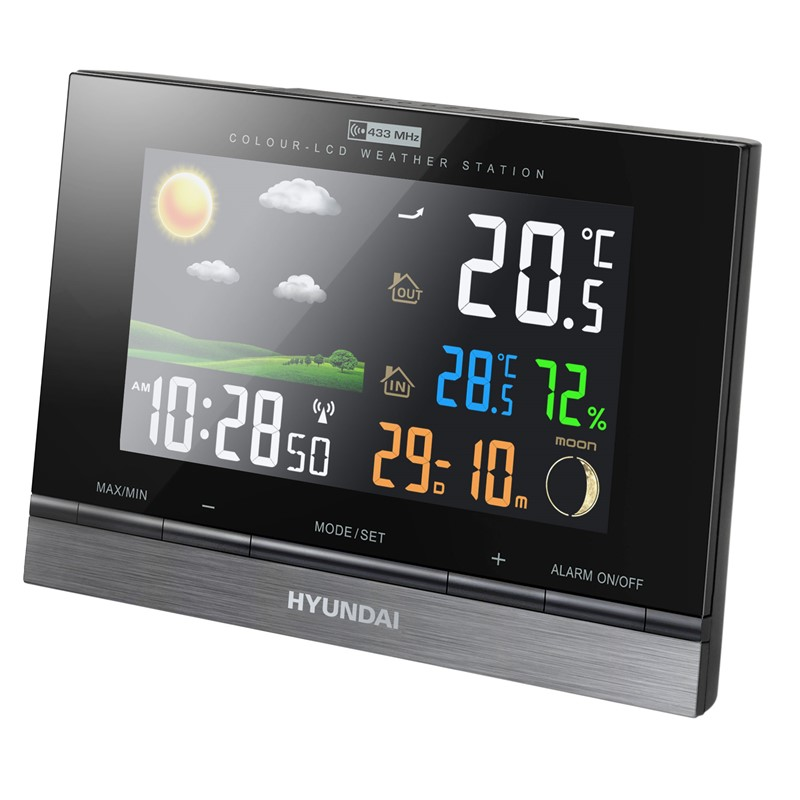
\includegraphics{LaTeX sablona IB/obrazky/hyundai.jpg}}
        \caption{meteostanice Hyundai WS 2303~\cite{WS2303Obrazek}}
        \label{hyundaiWS}
        \end{figure}

    \section{Sencor SWS 12500 WiFi}
        Základem meteostanice je hlavní jednotka, která nabízí přehledná data na displeji a uživatelská tlačítka (obr.~\ref{sencorWS}). K hlavní jednotce lze připojit až 7~bezdrátových vnitřních čidel, měřících teplotu a vlhkost a jednu venkovní jednotku 7v1, která měří teplotu, vlhkost, tlak, rychlost a směr větru, intenzitu světla, intenzitu UV záření a srážky. Naměřené údaje se prostřednictvím WiFi posílají do řídicí jednotky, která je zobrazuje a vytváří předpověď počasí na 12 až 24 hodin dopředu~\cite{SWS12500WIFI}.
        
        Veškerá data jsou dostupná online v mobilní aplikaci, meteostanice podporuje veřejné platformy Weathercloud, Weather Underground a Počasí Meteo, do kterých jsou zapojeni uživatelé z celého světa a přispívají daty ze svých stanic. Cena je 4799 Kč~\cite{SWS12500WIFI}.
        
        \begin{figure}[htb]
        \resizebox{8cm}{!}{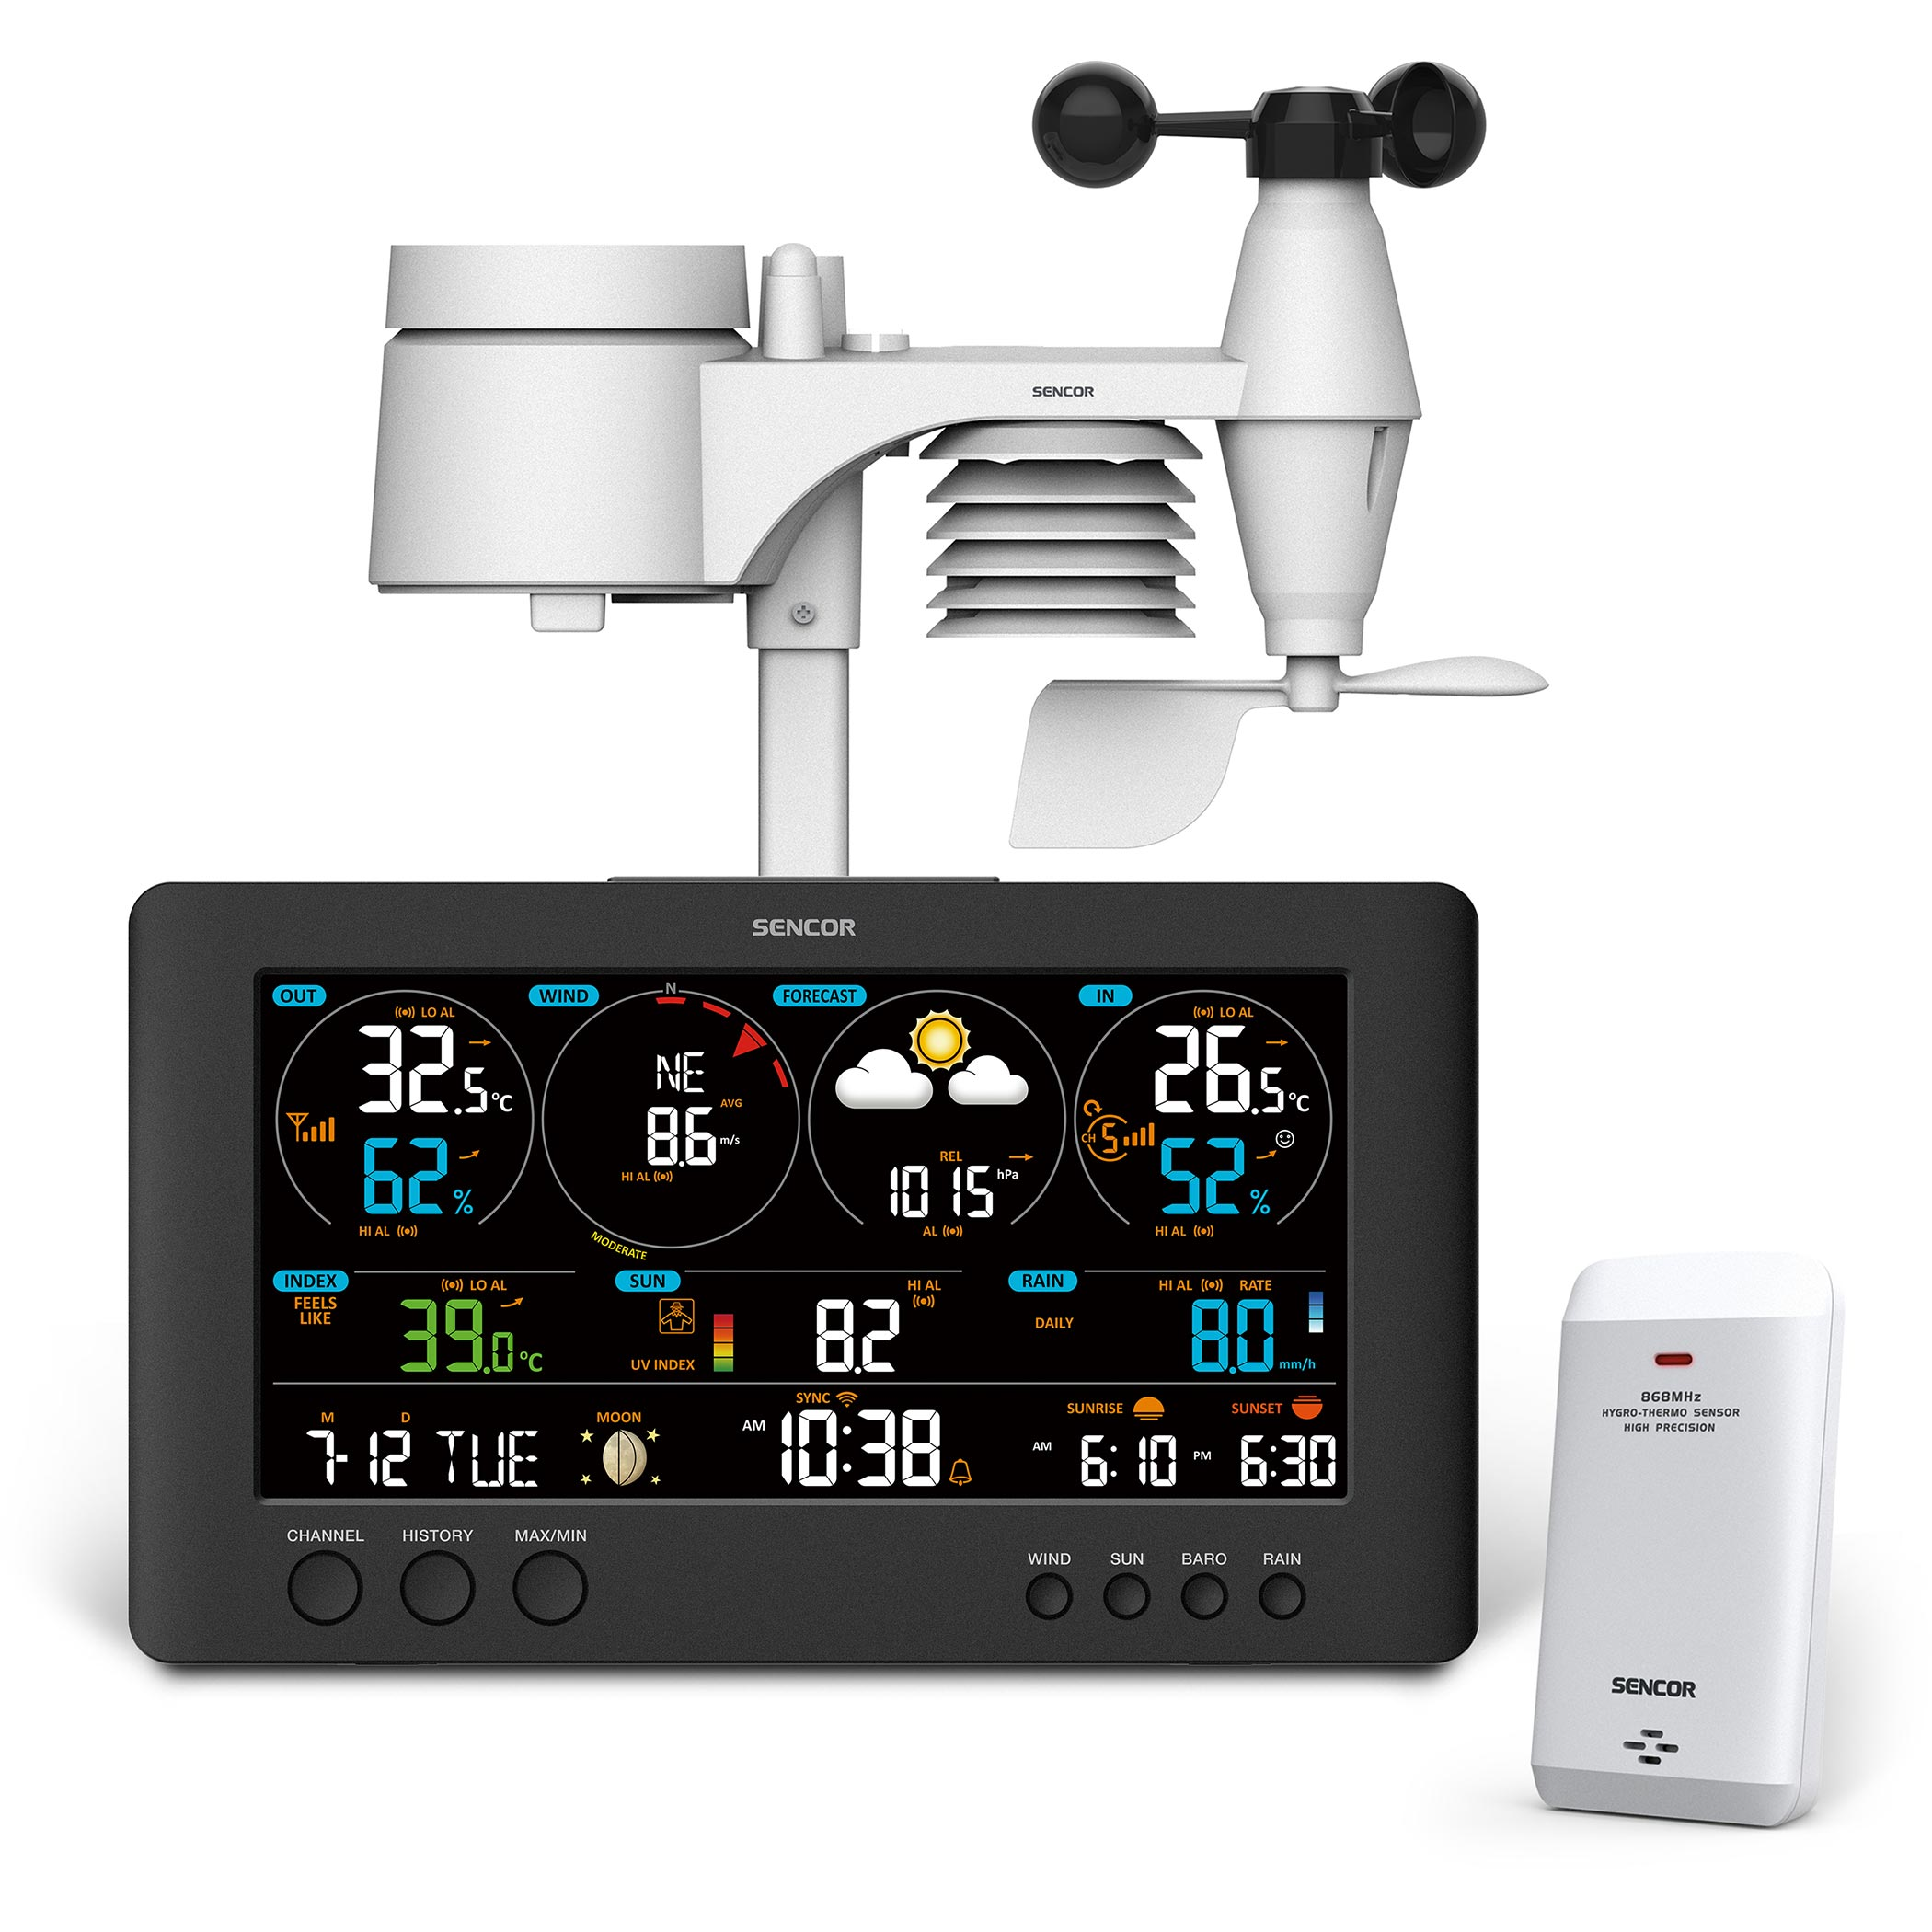
\includegraphics{LaTeX sablona IB/obrazky/sencor.jpg}}
        \caption{meteostanice Sencor SWS 12500 WiFi~\cite{SWS12500Obrazek}}
        \label{sencorWS}
        \end{figure}
        \chapter{Displeje}

    „\emph{V dnešní době jsou displeje a obrazovky naprosto neoddělitelnou součástí moderního života. Vždyť do nich koukáme po většinu každého dne!}~\cite{DisplejToply}“ Displej je zařízení, které zobrazuje informace (text, obrázky, znaky). Druhů displejů existuje opravdu spousta, například elektromechanické (překlápěcí, terčíkové, segmentové)~\cite{ElektromechanickeDispleje}, segmentové LED displeje a LED maticové displeje, LCD, OLED displeje, E-ink displeje a další. Základní parametry displejů jsou: úhlopříčka, rozlišení (počet pixelů, které dokáže zobrazit), obnovovací frekvence, odezva, jas a kontrast, barevná reprodukce a povrchová úprava~\cite{DisplejToply}.

    \section{Segmentové a maticové LED displeje}
        Segmentové displeje umožňují zobrazit číslice, znaky nebo symboly. Lze ovládat pouze jednotlivé segmenty, předurčené z výroby. Používají se v elektronických zařízeních, jako jsou měřící přístroje, hodiny, kalkulačky a další. Nejčastější typy jsou LCD segmentové displeje (viz obr.~\ref{LCDseg}) a LED segmentové displeje (viz obr.~\ref{LEDseg})~\cite{ZobrazovaciJednotky}.

        \begin{figure}[htb]
        \resizebox{8cm}{!}{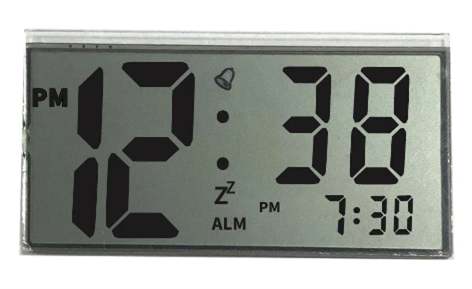
\includegraphics{LaTeX sablona IB/obrazky/LCD_seg_displej.png}}
        \caption{LCD segmentový displej~\cite{LCDsegDisplej}}
        \label{LCDseg}
        \end{figure}
        
        \begin{figure}[htb]
        \resizebox{8cm}{!}{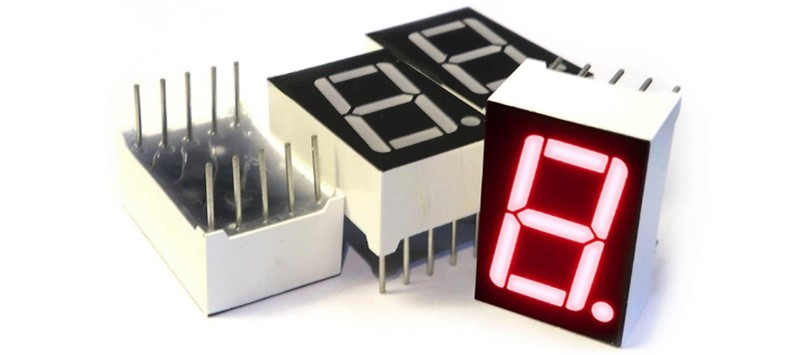
\includegraphics{LaTeX sablona IB/obrazky/LED_seg_displej.jpg}}
        \caption{LED 7 segmentový displej~\cite{7segmentdisplejPrincipAfunkcia}}
        \label{LEDseg}
        \end{figure}
        
        Maticové displeje se skládají z maticově uspořádaných LED. Používají se například jako informační tabule (viz obr.~\ref{LEDmat})~\cite{MaticovyLEDdisplej}.

        \begin{figure}[htb]
        \resizebox{8cm}{!}{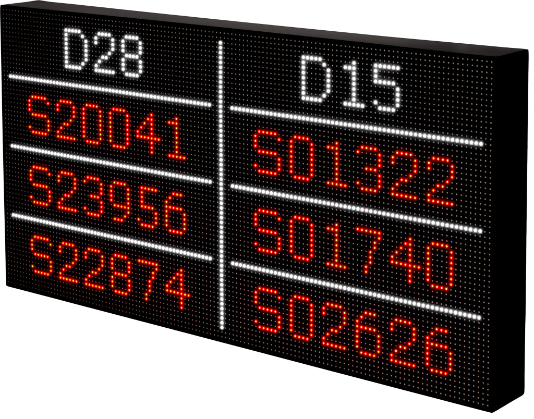
\includegraphics{LaTeX sablona IB/obrazky/maticovy_LED_displej.png}}
        \caption{maticový LED displej~\cite{MaticovyDisplej}}
        \label{LEDmat}
        \end{figure}

    \section{LCD}
        LCD (Liquid Crystal Display) funguje na principu tekutých krystalů, které jsou vloženy mezi dvě elektrody a polarizační filtry. Po připojení napájení na elektrody se uspořádání krystalů natáčí a tím mění své optické vlastnosti. U~barevných LCD se každý pixel dělí na 3 buňky - červenou, zelenou a modrou, přičemž u každé z nich lze díky natáčení krystalů zvlášť měnit jas.
        
        Využívají se jako obrazovky monitorů, televizí a různých přístrojů~\cite{DisplejeLCD}. Příklad takového displeje můžete vidět na obrázku~\ref{TFTLCD}. Na principu tekutých krystalů funguje také velká část segmentových displejů a znakových displejů s maticovými poli viz obr.~\ref{LCDalfn}. V dnešní době jsou větší obrazovky (ne ty segmentové) často nahrazovány OLED displeji - viz kapitola 2.3. Výhodou větších LCD obrazovek je, že jsou velmi ploché a mají poměrně nízkou spotřebu. Problémem těchto displejů je kontrast v tmavších barvách. Krystaly nedokáží zastavit všechno světlo, tudíž místo černé barvy zobrazí tmavý odstín šedé~\cite{ZobrazovaciGrafickaZarizeni}.

        \begin{figure}[htb]
        \resizebox{8cm}{!}{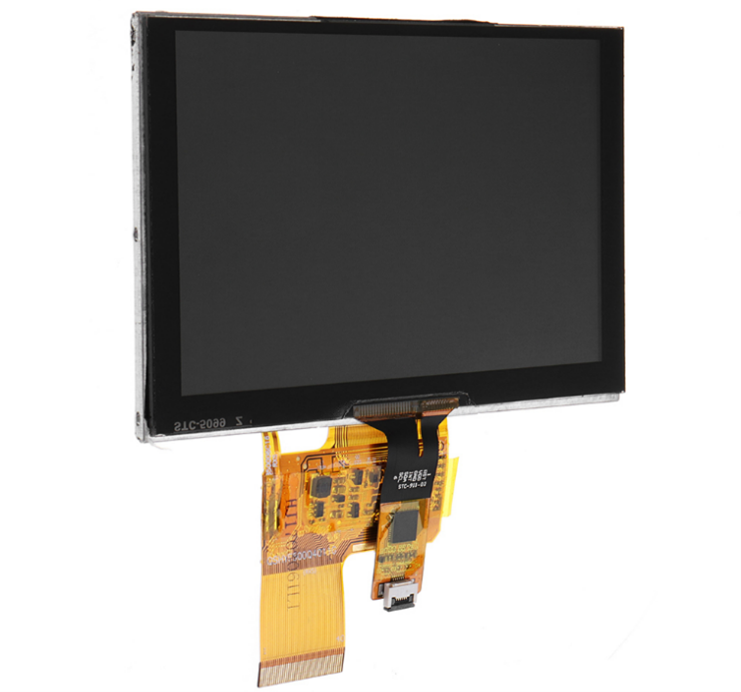
\includegraphics{LaTeX sablona IB/obrazky/LCD_TFT.png}}
        \caption{TFT LCD 800x480 dotykový~\cite{TFTLCDdisplej}}
        \label{TFTLCD}
        \end{figure}

        \begin{figure}[htb]
        \resizebox{8cm}{!}{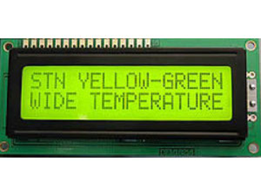
\includegraphics{LaTeX sablona IB/obrazky/LCD_alfn.png}}
        \caption{alfanumerický LCD~\cite{DisplejeLCD}}
        \label{LCDalfn}
        \end{figure}

    \clearpage

    \section{OLED displeje}
        OLED (Organic Light Emitting Diode) je jedna z nejnovějších zobrazovacích technologií. Využívá technologii organických elektroluminescenčních diod~\cite{ZobrazovaciGrafickaZarizeni}. Zde na rozdíl od LCD funguje každý pixel jako nezávislý zdroj světla. To umožňuje vyšší kontrast a úsporu energie. OLED displeje se používají v~mobilních telefonech, monitorech, televizích a v mnoha dalších přístrojích (obr.~\ref{OLED}). Nevýhodou těchto displejů je vypalování pixelů. Pokud bude pořád ve stejné části displeje dlouho svítit například nějaký znak, bude mírně vidět i po vypnutí obrazovky, nebo změně obrazu.

        \begin{figure}[htb]
        \resizebox{8cm}{!}{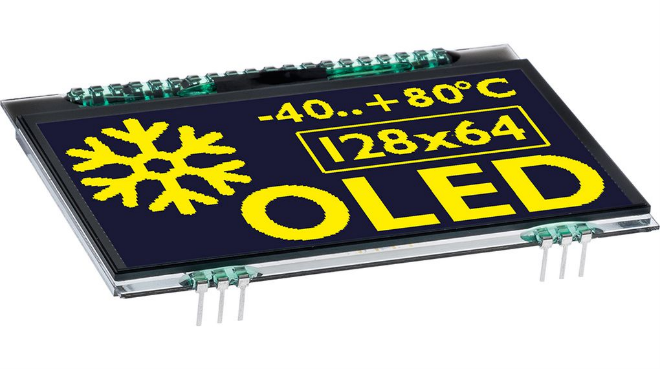
\includegraphics{LaTeX sablona IB/obrazky/oled.png}}
        \caption{OLED displej 128x64~\cite{OLEDDisplay}}
        \label{OLED}
        \end{figure}

    \section{E-ink displeje} \label{EinkKapitola}
        E-ink, E-paper, nebo také elektronický papír je technologie displeje, která se vzhledem velmi podobá klasickému papíru (obr.~\ref{EinkDisp}). Na rozdíl od většiny jiných způsobů zobrazování, kde jednotlivé pixely vyzařují světlo, zde pixely světlo pouze odráží (jako u obyčejného papíru s inkoustem). Tyto displeje jsou velmi úsporné, elektrickou energii potřebují jen při překreslení~\cite{EinkToply}. Takové překreslení ale většinou trvá kolem 1 až 3 sekund, proto nejsou vhodné pro aplikace, kde je potřeba rychlá obnovovací frekvence. Další nevýhodou je malá škála barev. Často mají k dispozici pouze pár odstínů šedé, avšak barevné displeje už také nejsou neobvyklé. Poměrně dlouhou dobu se používají v~elektronických čtečkách knih, nově také v supermarketech jako elektronické cenovky a začínají se objevovat v chytrých zařízeních jako jsou hodinky, mobilní telefony a monitory (viz obrázek~\ref{EinkMon}).

        \begin{figure}[htb]
        \resizebox{8cm}{!}{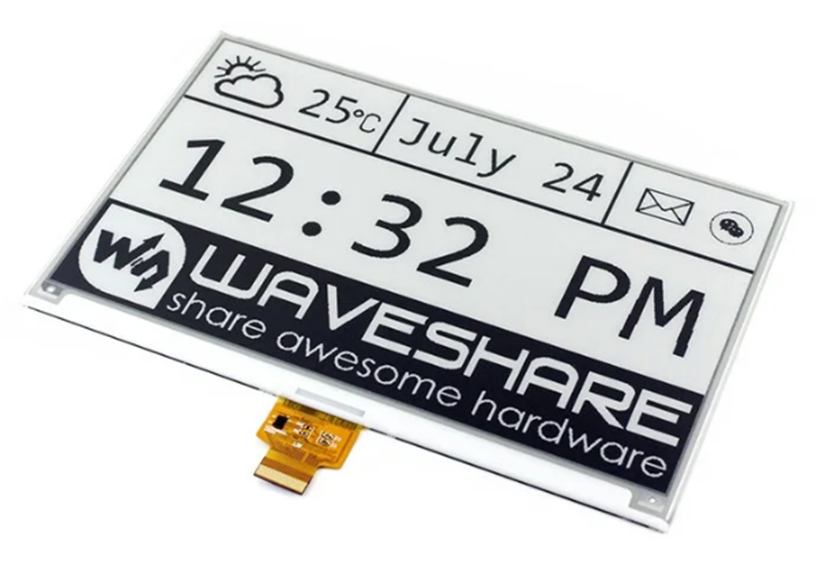
\includegraphics{LaTeX sablona IB/obrazky/eink_displej.png}}
        \caption{E-ink displej 7,5" 800x480px~\cite{E-Ink800x480px}}
        \label{EinkDisp}
        \end{figure}
        
        \begin{figure}[htb]
        \resizebox{8cm}{!}{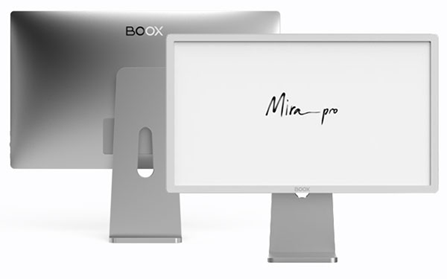
\includegraphics{LaTeX sablona IB/obrazky/eink_monitor.png}}
        \caption{E-ink monitor Onyx Boox Mira PRO, 25"~\cite{ONYXBOOXMIRAPRO}}
        \label{EinkMon}
        \end{figure}

        \chapter{Měření teploty}

    Měření teploty vzduchu je pro meteorologii a předpověď počasí velice důležité. Teplota vzduchu se měří pomocí teploměru. Teploměry se dělí na skupiny: dilatační teploměry, elektrické teploměry, speciální teploměry a bezdotykové teploměry. Skupina dilatačních teploměrů se dále dělí dle typu na: plynové, tenzní, kapalinové, kovové. Z nichž nejznámější jsou kapalinové, které měří objem kapaliny, jenž je závislý na teplotě. Sem patří například lihový, nebo pro profesionální měření častěji používaný rtuťový teploměr. Kapalinové teploměry jsou spolehlivé, přesné a levné, avšak jejich nevýhodou je křehkost a obtížnost dálkového přenosu údaje~\cite{Mereniteploty}. Další skupinou jsou elektrické teploměry, které se dále dělí na termoelektrické, odporové kovové, odporové polovodičové, diodové. Výstupem elektrických teploměrů je analogová hodnota v podobě elektrického napětí, které je na teplotě závislé podle určitého vztahu. Pro zpracování údaje digitálním zařízením se používají A/D převodníky.
    
    \section{Termoelektrické}
        Termoelektrické teploměry měří teplotu pomocí termoelektrických článků, které jsou vyrobeny z vodičů ze dvou různých kovů, které jsou vodivě spojeny. Při rozdílu teplot obou materiálů mezi nimi vzniká termoelektrické napětí. Zjednodušeně lze závislost termoelektrického napětí na teplotě vyjádřit lineárním vztahem. Jednotlivé termočlánky se označují velkými písmeny. Nejpoužívanější jsou články s označením T, J, X, S~\cite{Mereniteploty}.
        
    \section{Odporové}
        Odporové teploměry se dělí na kovové a polovodičové. Kovové teploměry se vyrábí výhradně z čistých kovů. Vhodné materiály jsou například platina, nikl a měď, z nichž nejpoužívanější je díky jednodušší výrobě a její fyzické i chemické stálosti platina. Na materiálu také záleží kvůli teplotnímu součiniteli. Ten by ideálně měl být stálý a co největší. Platina je výhodná také díky jejímu z ostatních materiálů nejvyššímu měřícímu rozsahu (-200 až 850 °C)~\cite{Mereniteploty}.
        
        Druhou skupinou odporových teploměrů jsou polovodičové, které se dále dělí na NTC-termistory, PTC-termistory a monokrystalické senzory teploty. Asi nejznámějším typem jsou NTC-termistory. Vyrábí se spékáním oxidů a důležité je, že závislost odporu na teplotě není lineární. Odpor s rostoucí teplotou klesá podle určitého vztahu~\cite{Mereniteploty}. Pro určení teploty podle elektrického odporu NTC-termistoru je potřeba znát β koeficient a daný odpor termistoru při teplotě 25 °C. β koeficient lze vypočítat, pokud známe odpor termistoru alespoň při dvou různých teplotách.

        \chapter{Stanovení návrhových parametrů}

    Cílem práce je navrhnout, sestavit a naprogramovat meteostanici vhodnou pro domácí použití. Meteostanice by měla měřit základní meteorologická data, ukládat je na mikro SD kartu a zobrazit je na displeji a na webserveru.
    
    Chtěl bych, aby venkovní jednotka, která bude měřit teplotu, vlhkost, tlak a rychlost větru, mohla s vnitřní jednotkou, měřící teplotu, vlhkost a koncentraci $CO_2$ komunikovat alespoň do vzdálenosti 50 m. Požadavky na akumulátor jsou: nízké samovybíjení, vysoká škála pracovní teploty (-15~až~50~°C). Venkovní jednotka bude napájena pouze ze 2W solárního panelu, tudíž je nutné zvolit dostatečnou kapacitu akumulátoru, aby dokázala vydržet přes noc a při oblačnosti. Pro vnitřní jednotku jsem zvolil napájení ze síťového adaptéru, mělo by stačit 5 V a 1 A.
    
    Pro vnitřní jednotku použiji 3D vytištěnou krabičku/stojánek, kde budou otvory pro napájení, mikro SD kartu a velký výřez pro displej. Konstrukce venkovní jednotky se bude skládat z vodotěsné instalační krabice (pro DPS a akumulátor), anemometru pro měření rychlosti větru, radiačního krytu se senzorem teploty i vlhkosti a solárního panelu uchyceného nad instalační krabicí. Na DPS v instalační krabici bude senzor tlaku a teploty, rádiový vysílač a solární nabíječka.
        \chapter{Praktická část}
    V této kapitole se budu věnovat postupem návrhu a výroby od samého začátku až do konečné fáze projektu. Zaměřím se na konstrukční, elektrickou i programovou část projektu a zmíním funkce, části a vlastnosti, se kterými jsem spokojený. Pozastavíme se i nad chybami, kterých nebylo málo a věcmi, které by se daly v budoucnu vylepšit.

    \section{Konstrukční část} \label{KonstCast}
        Jako všechny ostatní části se i konstrukční dělí na vnitřní a venkovní. V této podkapitole podrobně popíši postup návrhu, výroby i sestavení všech dílčích částí meteostanice. Při návrhu všech 3D objektů a sestav jsem pracoval v programu Autodesk Fusion 360 verze 2.0.18460~\cite{AutodeskFusion360} a všechny 3D-tištěné díly jsem navrhnul a vymodeloval. Stažené modely jsou pouze kabelové průchodky, oba mikrokontrolery ESP32, BMP280, DHT22 a MH-Z19B.

        \begin{figure}[htb]
        \resizebox{13cm}{!}{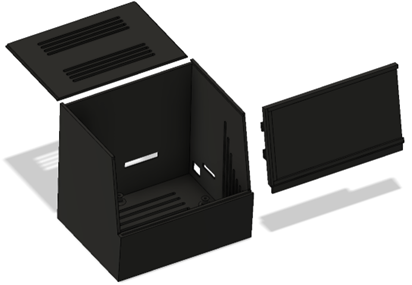
\includegraphics{LaTeX sablona IB/obrazky/VnitrniKrabicka.png}}
        \caption{Krabička vnitřní jednotky meteostanice}
        \label{Krab}
        \end{figure}

        Pro vnitřní jednotku jsem vyráběl jen jednu verzi krabičky, kterou lze vidět na obrázku~\ref{Krab}. Při testování na nepájivém poli a testování různých verzí plošných spojů jsem pracoval bez konstrukčních prvků (bez krabičky). Návrh krabičky mi zabral poměrně dost času, hlavním problémem bylo umístění a přidělání displeje, protože je tenký a křehký. 3D tištěné díly bylo potřeba obrousit a upravit, ale s tím jsem musel počítat. Krabička se skládá ze 3 částí – samotná krabička, díl pro uchycení displeje a víko. V krabičce i ve víku jsou větrací otvory pro proudění vzduchu kvůli senzoru $CO_2$ a senzoru teploty. Dále se zde nachází otvor pro napájecí kabel microUSB, otvor pro budoucí připojení externího NTC čidla teploty, pro které ale zatím není uzpůsoben program a otvor pro vložení microSD karty. Sloupky, na které se přišroubuje deska plošných spojů, jsou zde kvůli uspořádání součástek na plošném spoji pouze tři. Pro díry ve sloupcích je nutné zvolit menší průměr, aby se při šroubování mohl vytvořit závit. Všechny tři části vnitřní krabičky jsem tisknul z černého materiálu PLA, protože je dostupný a jeho vlastnosti na toto využití postačí. Následně jsem ořezal a~obrousil místa, která do sebe mají pasovat, a vše poskládal.

        Pro konsrukci venkovní části meteostanice jsem kvůli jejich lehkosti, pevnosti a odolnosti proti korozi zvolil duté čtyřhranné hliníkové tyče o délce strany 15 mm a tloušťce hliníku 1 mm. Z takovýchto 5 různě dlouhých tyčí je tvořena základní kostra meteostanice, na kterou je přidělána ústředna a~jednotlivé prvky se senzory. Hliníkové tyče jsou k sobě přišroubovány pozinkovanými šrouby a samojistnými maticemi M5. Pro možnost lepšího utáhnutí jsem použil i pozinkované podložky. Vrstva zinku chrání šrouby, matice a~podložky před korozí. Kostra z dutých hliníkových tyčí umožňuje vedení vodičů uvnitř konstrukce, díky tomu jsou chráněny před deštěm a UV zářením a přispívá to k čistějšímu vzhledu. Konce hliníkových tyčí jsou opatřeny tištěnými plastovými krytkami.
        \newpage

        \subsection{Ústředna}    
            Ústřednu tvoří bílá vodotěsná instalační krabice S-BOX 416 o rozměrech 190 x 140 x 70 mm se stupněm krytí IP 65, tudíž je elektronika uvnitř chráněna před UV zářením, prachovými částicemi a samozřejmě před deštěm. Pro vstup vodičů do ústředny jsem zvolil kabelové průchodky M20, které se dají utáhnout a brání tak vniku vody a vlhkosti do krabice. Pro tyto průchodky bylo potřeba vyvrtat 2 otvory o průměru 20 mm. Ústředna je k hliníkové konstrukci přidělána pozinkovanými šrouby M5 s těsnící páskou. Pro upevnění elektronických komponent do krabice jsem navrhl desku s otvory na šroubky, sloupky pro přidělání plošného spoje a otvory na stahovací pásky, kterými se upevní akumulátor a kabely, viz obrázek~\ref{Deska}. Tato deska je také vytištěna na 3D tiskárně z bílého materiálu PETG.

            \begin{figure}[htb]
            \resizebox{10cm}{!}{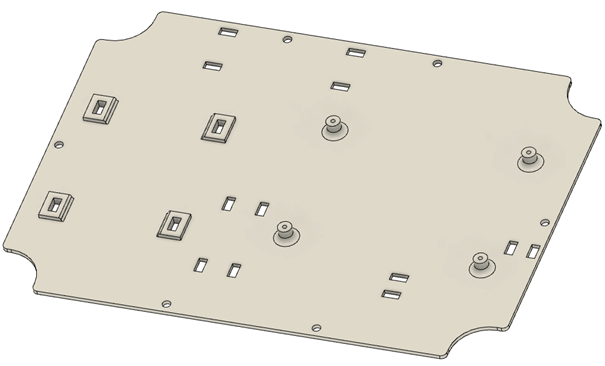
\includegraphics{LaTeX sablona IB/obrazky/DeskaProUpevneniElektroniky.png}}
            \caption{Deska pro upevnění elektroniky}
            \label{Deska}
            \end{figure}

        \subsection{Uchycení solárního panelu}
            Solární panel je důležité umístit tak, aby byl chráněn před deštěm a kroupami, ale také aby se k němu dostávalo co nejvíce světla po co nejdelší dobu. Pro přidělání solárního panelu jsem použil 3D tištěné komponenty, plexisklo o~tloušťce 3 mm, pozinkované šrouby, matičky a podložky. Celá sestava je na obrázku~\ref{SestavaPanel}. Do hlavního plastového dílu jsem vložil panel a protáhl kabel otvorem. Na tento hlavní díl jsem lepidlem na plexisklo přilepil obdélník plexiskla vyřezaný na laseru. Po zaschnutí lepidla jsem mohl protáhnout kabel hliníkovou konstrukcí a kabelovou průchodkou až do instalační krabice a přichytit panel ve vyrobeném krytu na vrchní vodorovnou tyč pomocí tištěných dílů (obrázek~\ref{DilyPanel}) a čtyř šroubů. Panel je od konstrukce nakloněný pod úhlem 45°, což asi vzhledem k pozdějšímu umístění meteostanice není nejlepší možný úhel, ale je to takhle konstrukčně jednodušší. Pro pevnost uchycení je důležité, aby se díl, který objímá tyč zespoda tisknul bokem (tak aby síla při dotáhnutí šroubů neodtahovala jednotlivé vrstvy od sebe).

            \begin{figure}[htb]
            \resizebox{10cm}{!}{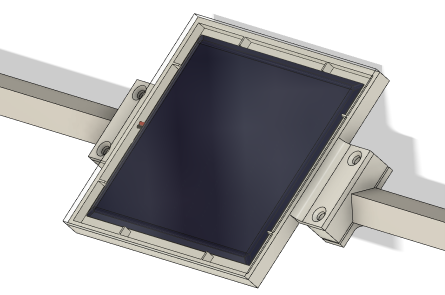
\includegraphics{LaTeX sablona IB/obrazky/SestavaKrytuNaPanel.png}}
            \caption{Sestava krytu na panel}
            \label{SestavaPanel}
            \end{figure}

            \begin{figure}[htb]
            \resizebox{6cm}{!}{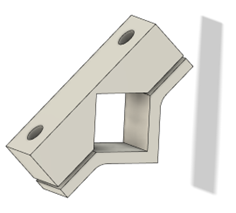
\includegraphics{LaTeX sablona IB/obrazky/UchyceniPanelu.png}}
            \caption{Díly pro uchycení panelu na konstrukci}
            \label{DilyPanel}
            \end{figure}

        \clearpage

        \subsection{Konstrukční/mechanická část anemometru}
            Anemometr (obrázek~\ref{Anemometr}) je součást meteostanice, která měří rychlost větru. Skládá se ze: 3 tištěných dílů, ložiska, senzoru a dvou neodymových magnetů o~rozměrech 3 x 2,5 x 1 mm. Rotační část tvoří vrtulka se třemi kulovými kalíšky, které mají díky svému tvaru menší odpor vzduchu ve směru otáčení, než proti směru. Zevnitř rotační části se nachází magnety umístěné naproti sobě. U anemometru je důležité, aby byl umístěný v prostoru kvůli otáčení vrtulky. Při navrhování vrtulky jsem nejprve zvolil vzdálenost kalíšků od středu 35~mm a jejich vnitřní poloměr 12 mm. To se později ukázalo jako neefektivní a pro druhý a zároveň poslední model vrtulky jsem použil vzdálenost kalíšků od středu 60 mm a jejich vnitřní poloměr 20 mm. S~výsledkem jsem spokojený, vrtulka je v rámci možností pevná a točí se s~poměrně malým odporem. Pod rotační částí se nachází pevný díl se senzorem, ze stran utěsněným silikonem proti vodě. Tento pevný díl, na kterém je nasazené ložisko s rotační částí, je stahovacími páskami připevněn k vrchní vodorovné tyči konstrukce. Vnitřkem pevné části anemometru prochází kabel od senzoru, který z vrchu vstupuje do hliníkové konstrukce, prochází až k~instalační krabici a vstupuje kabelovou průchodkou k řídicí jednotce.

            \begin{figure}[htb]
            \resizebox{10cm}{!}{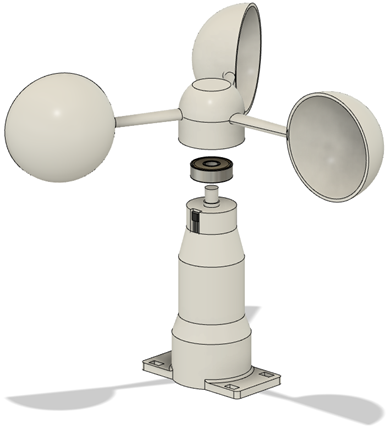
\includegraphics{LaTeX sablona IB/obrazky/Anemometr.png}}
            \caption{Anemometr}
            \label{Anemometr}
            \end{figure}

        \clearpage

        \subsection{Radiační kryt}
            Radiační kryt, který můžete vidět na obrázcích~\ref{RadSestava},~\ref{RadPostup} a~\ref{RadVysledek} chrání senzor teploty a vlhkosti před slunečním zářením a před deštěm. Je navržen tak, aby v něm bylo možné měřit teplotu s co nejmenší chybou, i když je na slunci. Pro jeho výrobu jsem použil závitovou tyč M4, kterou jsem nařezal na 3 stejně dlouhé kusy po 10 cm a plastové kruhové díly vytisknuté z bílého PETG. Tyto plastové „lamely“ musí být  navrženy tak, aby dostatečně chránily senzor před slunečním zářením a před deštěm, ale aby jimi zároveň co nejlépe proudil vzduch. Závitové tyče jsou upevněny k vrchní stříšce a na ně se postupně navlékají kruhové obroučky střídavě s distančními sloupky. Místo jednoho sloupku jsem umístil úchyt s otvorem pro přidělání senzoru. Jako poslední je navlečený díl pro uchycení k horní tyči konstrukce a vše je utáhnuto samojistnými maticemi. Spodní díl je ke konstrukci stejně jako anemometr přidělán dvěma stahovacími páskami.

            \newpage

            \begin{figure}[htb]
            \resizebox{3.5cm}{!}{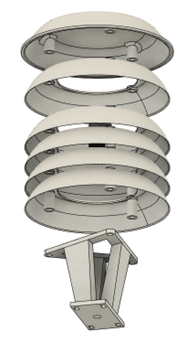
\includegraphics{LaTeX sablona IB/obrazky/RadiacniKrytSestava.png}}
            \caption{Radiační kryt: sestava}
            \label{RadSestava}
            \end{figure}

            \begin{figure}[htb]
            \resizebox{3.5cm}{!}{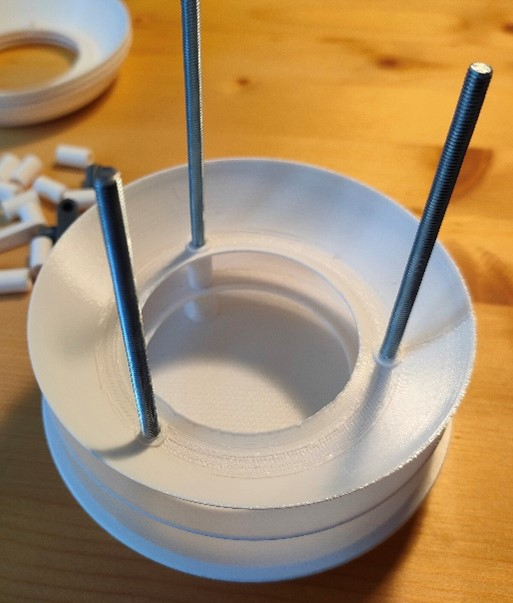
\includegraphics{LaTeX sablona IB/obrazky/RadiacniKrytVyroba.jpg}}
            \caption{Radiační kryt: postup výroby}
            \label{RadPostup}
            \end{figure}

            \begin{figure}[htb]
            \resizebox{3.5cm}{!}{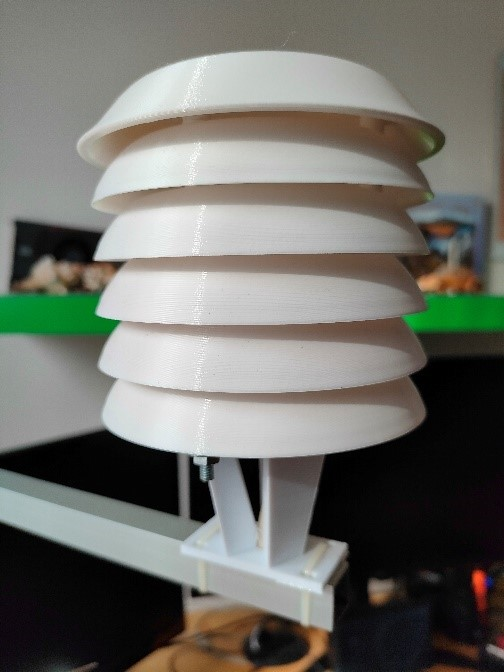
\includegraphics{LaTeX sablona IB/obrazky/RadiacniKrytVysledek.jpg}}
            \caption{Radiační kryt: výsledek}
            \label{RadVysledek}
            \end{figure}

    \clearpage

    \section{Elektrická část} \label{ElCast}
        Tato kapitola se zabývá výběrem, návrhem a realizací všech elektronických komponent vnitřní i venkovní jednotky meteostanice. Při návrhu plošných spojů jsem pracoval v programu KiCad 7.0~\cite{KiCad} a při jejich výrobě v učebně 124. Plošným spojům však předcházelo testování na nepájivém poli, viz obrázek~\ref{NepajivePole}. V následujících podkapitolách podrobně popíši postup při výrobě jednotlivých elektrických částí.

        \begin{figure}[htb]
        \resizebox{12cm}{!}{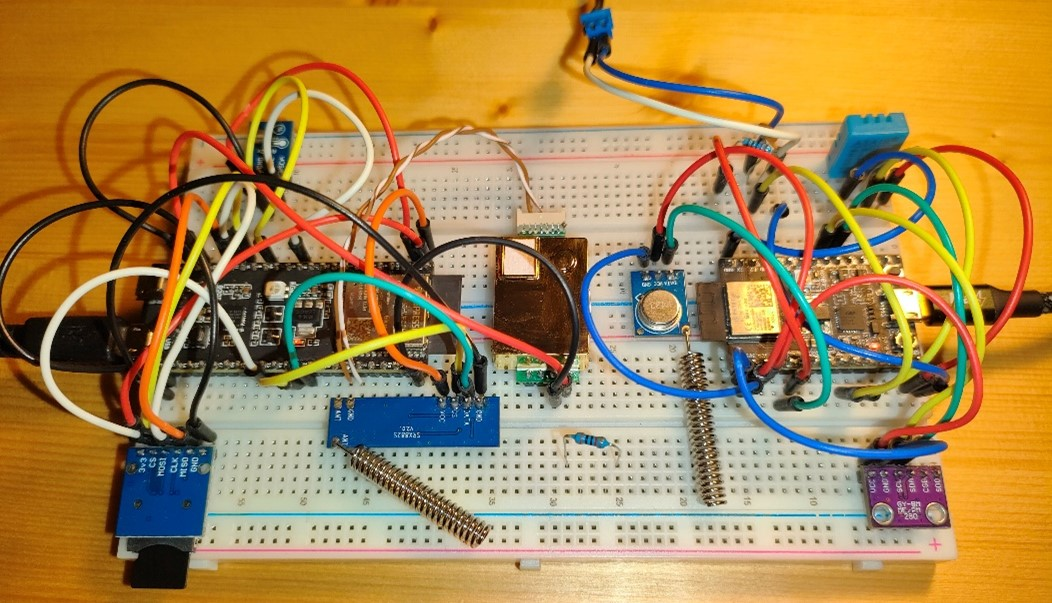
\includegraphics{LaTeX sablona IB/obrazky/ZapojeniNaNepajivemPoli.jpg}}
        \caption{Zapojení na nepájivém poli}
        \label{NepajivePole}
        \end{figure}

        \subsection{Vnitřní jednotka} \label{ElVnitrniJednotka}
            Elektroniku vnitřní jednotky tvoří plošný spoj, na kterém se nachází hlavní řídicí jednotka ESP32s3, rádiový přijímač NiceRF 433 MHz, senzor $CO_2$, senzor teploty a vlhkosti, modul pro mikroSD kartu, vývody pro displej a konektor pro budoucí připojení externího NTC čidla teploty. ESP32s3 jsem zvolil jako hlavní řídicí jednotku kvůli jeho dostatečnému počtu pinů, možnosti připojení k wifi a dalším funkcím. Pro měření koncentrace $CO_2$ ve vzduchu jsem pořídil MH-Z19B hlavně kvůli jeho dostupnosti a rozsahu měření (0 až 5000 ppm). Dále jako modul měření teploty a vlhkosti jsem vybral AHT21, protože je dostatečně přesný, malý a komunikuje přes sběrnici I$^2$C. Komunikaci mezi vnitřní a venkovní jednotkou zajišťují rádiové moduly NiceRF 433 MHz. Pro tuto aplikaci jsou ideální díky svému dosahu a nízké spotřebě. Displej jsem zvolil typu E-ink, konkrétně 3,7" GDEY037T03, protože se mi líbí a myslím, že se pro tento projekt hodí. Detailně jsem tento typ displejů popisoval v kapitole~\ref{EinkKapitola} s názvem E-ink displeje.

            Plošných spojů do vnitřní části jsem vyráběl několik verzí, vždy jsem něco přidal, nebo změnil rozvržení součástek. Většinu plošných spojů jsem leptal. Vyzkoušel jsem i vyrábění na frézce, ale leptané spoje se ukázaly jako lepší a spolehlivější. Poslední a použitá verze je na obrázcích~\ref{DPSosazena} a \ref{DPSpajeni}. Detailnější informace ke všem použitým plošným spojům naleznete v příloze pod názvem Dokumentace DPS.

            \begin{figure}[htb]
            \resizebox{8cm}{!}{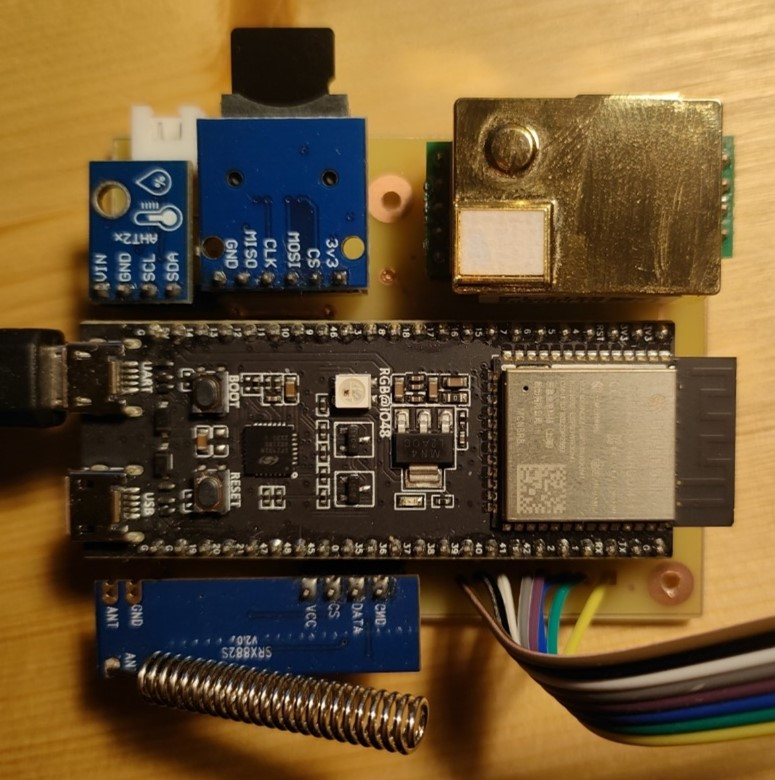
\includegraphics{LaTeX sablona IB/obrazky/OsazenaDPSvnitrni.jpg}}
            \caption{Osazená DPS}
            \label{DPSosazena}
            \end{figure}

            \begin{figure}[htb]
            \resizebox{8cm}{!}{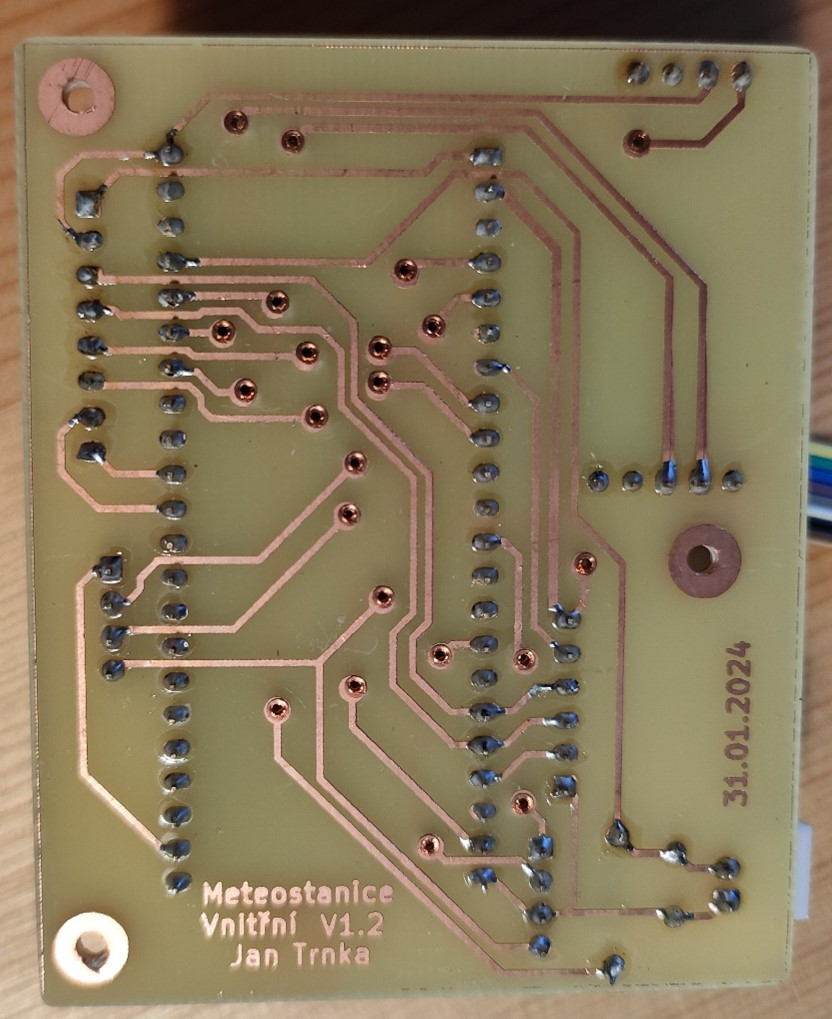
\includegraphics{LaTeX sablona IB/obrazky/OsazenaDPSzeStranyPajeniVnitrni.jpg}}
            \caption{Osazená DPS ze strany pájení}
            \label{DPSpajeni}
            \end{figure}

        \clearpage

        \subsection{Venkovní jednotka}
            Elektroniku ve venkovní části řídí mikrokontroler ESP32c3, který je umístěný na plošném spoji spolu s modulem pro nabíjení akumulátoru ze solárního panelu a napájení 5 V. Dále se tam nachází senzor tlaku a teploty BMP280, rádiový vysílač NiceRF 433 MHz a trubičková pojistka na 200 mA. Všechny moduly jsou na desku připojené přes DuPont dutinkové lišty, aby se daly v~případě potřeby vyjmout nebo vyměnit. Zjistil jsem, že obyčejné trubičkové pojistky na nižší proud (např. na 40 mA) mají odpor kolem 70 Ω, takže jsou při tak malém napětí nepoužitelné. Venkovní jednotka odebírá při DeepSleep módu kolem 9 mA, v normálním režimu 34–36 mA a při odesílání dat, což trvá méně než 1 s, je nejvyšší proud 60 mA. Dále jsou na plošném spoji JST konektory pro připojení akumulátoru a NTC čidla pro měření teploty. Ani v této jednotce však není program připravený na jeho použití, ale tady k~tomu nevidím zásadní důvod. Vodiče z anemometru, senzoru DHT22 a ze solárního panelu jsou připojeny do dvou a tří pinových svorkovnic s roztečí 2,54 mm. Kabely pro komunikaci s anemometrem a senzorem DNT22 jsem použil CAT5e UTP a přebytečné vodiče nejsou nikam zapojeny. Akumulátor se skládá ze 6 Li-ion článků SE US18650GR o udávané kapacitě $2600$ mAh. Při průměrném odběru 13 mA by měla venkovní jednotka teoreticky vydržet bez nabíjení 50 dní. Reálně se dá počítat tak s polovinou, i kvůli tomu, že články nejsou nové, ale i tak si myslím, že je to dostačující. Na obrázku~\ref{Ustredna} lze vidět celou ústřednu s elektronikou a akumulátorem. Dále pak na obrázcích~\ref{A3144} a \ref{DHT22} zapojení anemometru a DHT22. Pro snímání magnetů v anemometru jsem použil Hallův senzor A3144 a oproti zapojení na obrázku 5.13 je napájený 3,3 V místo 5 V.

            \begin{figure}[htb]
            \resizebox{12cm}{!}{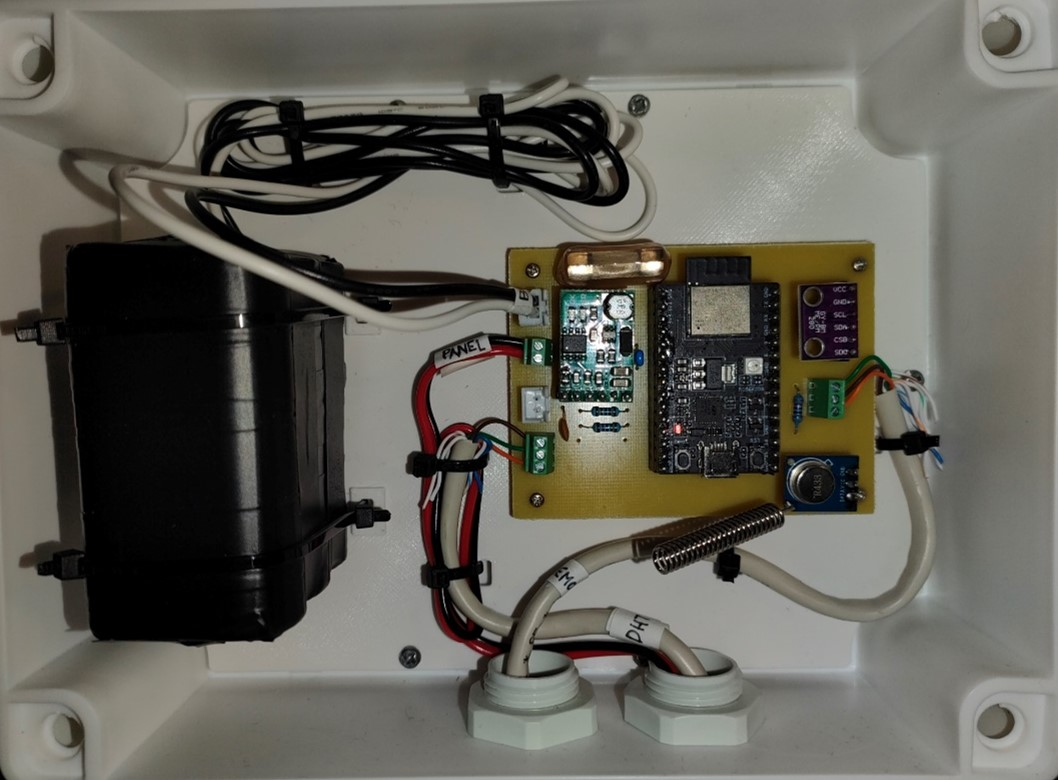
\includegraphics{LaTeX sablona IB/obrazky/Ustredna.jpg}}
            \caption{Ústředna}
            \label{Ustredna}
            \end{figure}

            \begin{figure}[htb]
            \resizebox{10cm}{!}{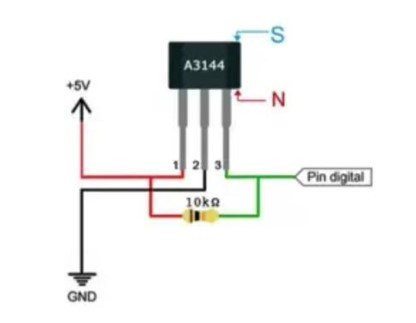
\includegraphics{LaTeX sablona IB/obrazky/A3144Zapojeni.jpg}}
            \caption{Vzorové zapojení senzoru A3144~\cite{A3144Hall}}
            \label{A3144}
            \end{figure}

            \begin{figure}[htb]
            \resizebox{12cm}{!}{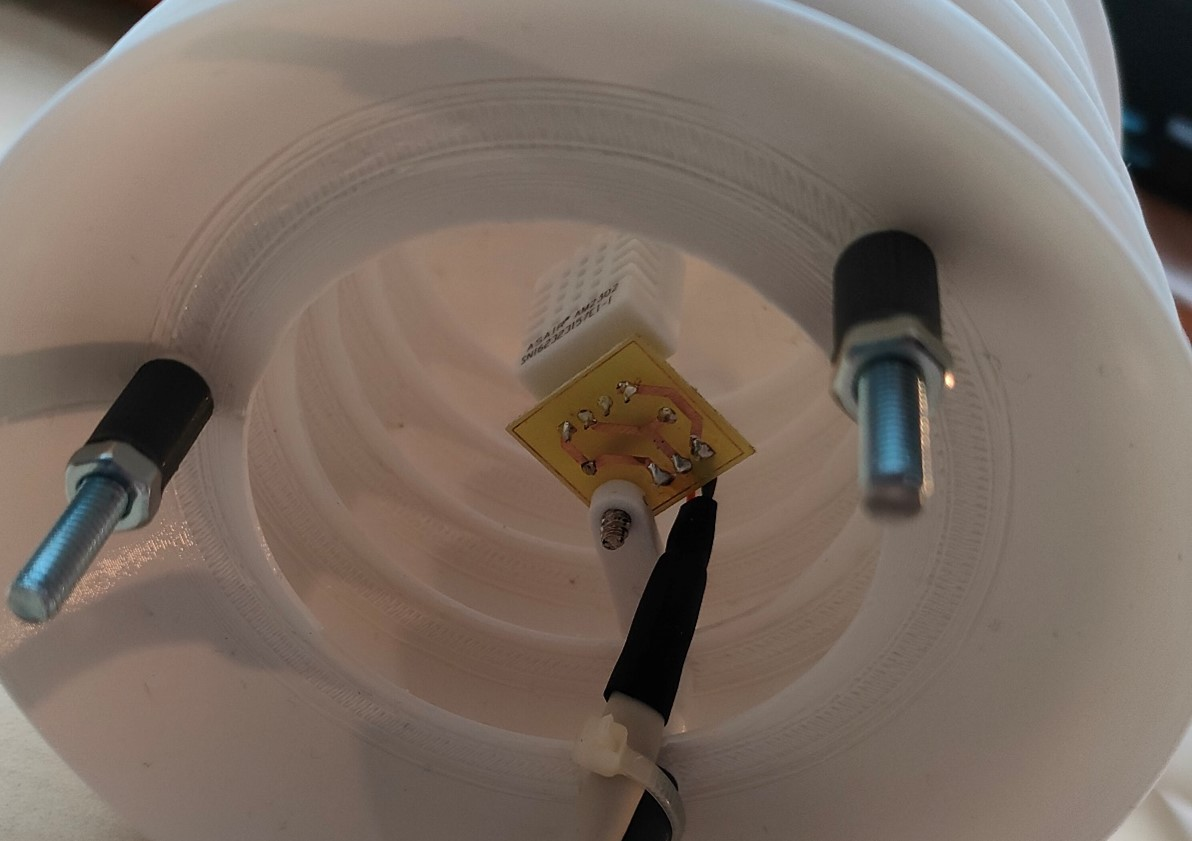
\includegraphics{LaTeX sablona IB/obrazky/DHT22naDPS.jpg}}
            \caption{Plošný spoj s DHT22 a rezistorem}
            \label{DHT22}
            \end{figure}

        \clearpage

    \section{Programová část} \label{PrgCast}
        Programování meteostanice mi ze všech částí jednoznačně zabralo nejvíce času. Nejdříve jsem testoval různé prvky a senzory zvlášť a po nějaké době je dával dohromady s dalšími. Při programování mi hodně pomohlo rozdělení programu do více souborů, bez toho si to už ani nedokáži představit. Hlavně u vnitřní jednotky je kód už poměrně veliký. Při programování jsem využíval Arduino IDE 2.3.2~\cite{ArduinoIDE}, při kreslení a generování souborů pro displej Adobe Illustrator 2023~\cite{Illustrator} a Image2Lcd~\cite{Image2Lcd}. V následujících podkapitolách se pokusím popsat fungování programu a jeho tvorbu.

        \subsection{Program venkovní jednotky}
            Začnu programem běžícím na venkovním ESP32c3, protože je jednodušší. K~hlavnímu souboru jsou připojeny 3 hlavičkové soubory – jeden pro BMP280 a DHT22, druhý pro rádiový modul a třetí obsahuje funkce pro výpočet rychlosti větru podle pulzů z anemometru. Při každém pulzu se zaznamenává pouze nástupná hrana. Měření rychlosti větru trvá obvykle 1 minutu. Pokud však není zaznamenán žádný impulz po dobu 30 sekund, měření se přeruší kvůli úspoře akumulátoru, odešlou se data a ESP32c3 se přepne do režimu spánku. Během měření se zaznamenává počet pulzů a doba mezi nimi. Z~nejkratší doby mezi pulzy se na konci vypočítá nejsilnější náraz větru. Po uplynutí jedné minuty se vypočítá průměrná doba mezi pulzy a z ní průměrná rychlost větru. Tato vypočítaná rychlost je však pouze teoretická. V reálném prostředí totiž nikdy nebude rychlost otáčení vrtulky stejná, jako rychlost větru. Proto se používá kalibrační konstanta, kterou lze vypočítat z vlastností vrtulky a vzduchu (například hmotnost a tvar vrtulky, hustota vzduchu, relativní vlhkost vzduchu, atmosférický tlak a další. Tento výpočet je však poněkud komplikovaný, proto jsem tuto konstantu určil pomocí vypůjčeného měřícího přístroje. Více o této kalibraci popíši v kapitole~\ref{Vyhodnoceni} s názvem Vyhodnocení. Pro senzory teploty, vlhkosti a tlaku používám knihovny Wire.h~\cite{Wire}, \hbox{Adafruit\_Sensor.h}~\cite{AdafruitSensor}, \hbox{Adafruit\_BMP280.h}~\cite{AdafruitBMP280Library} a~DHT.h~\cite{DHTsensorLibrary}, Pro rádiovou komunikaci potom \hbox{RH\_ASK.h}~\cite{RHASK}.

            Na začátku programu jsou zahrnuté všechny hlavičkové soubory a je zde definovaný čas pro hluboký spánek. Dále jsou deklarovány proměnné pro naměřené hodnoty datového typu float a následuje samotná funkce void setup(), ve které se na začátku nastaví potřebné piny jako vstupy. Spustí se funkce \hbox{bmp\_dht\_SETUP()}, ve které se zahájí komunikace přes I$^2$C a zkontroluje připojení senzorů BMP280 a DHT22. Následuje podobná funkce \hbox{NiceRF\_SETUP()}, v níž se inicializuje rádiový modul pro vysílání. Dále je na řadě funkce ReadWindSpeed(), ve které se po nastavený čas \hbox{READING\_TIME} zaznamenávají nástupné hrany pulzů ze senzoru A3144 a~doba mezi nimi. Po uplynutí nastaveného času se vypočítá průměrná rychlost větru. Během nastaveného času se také ukládá nejkratší doba mezi pulzy (náraz větru). Za funkcí ReadWindSpeed() už je jen ReadSendData(), kde se naměří data z ostatních senzorů a napětí akumulátoru a vše se odešle přes rádiový modul funkcemi radioSend() s parametry. První parametr datového typu char je znak, který slouží k rozpoznání hodnoty ve vnitřní jednotce, každá hodnota má jiný znak (a až g). Druhý parametr datového typu float nese naměřenou nebo v případě napětí akumulátoru a rychlosti větru vypočítanou hodnotu. Nyní je vše naměřeno a odesláno, takže už se jen nastaví časovač pro vzbuzení a ESP se přepne do režimu hlubokého spánku. Po uběhnutí časovače se vzbudí a celá funkce void setup() proběhne znovu. Funkce void loop() v~tomto programu není využita (je prázdná).

            \newpage

        \subsection{Program vnitřní jednotky}
            V programu vnitřní jednotky se  zpracovávají všechna data, ať už byla naměřena venku či vevnitř. Běží zde webserver, data se zapisují na mikroSD kartu a~vypisují se na displej. Zatímco na webserveru najdete veškerá data, se kterými meteostanice pracuje (kromě historie, která je na paměťové kartě), na displeji jsou pouze 4 základní hodnoty. To by se určitě dalo vylepšit větším displejem, kvůli ceně jsem ale vybral menší, 3,7" (konkrétněji v~kapitole~\ref{ElVnitrniJednotka} pod názvem Vnitřní jednotka). Na displeji se tedy zobrazují pouze: teplota uvnitř, teplota venku, koncentrace $CO_2$ a atmosférický tlak přepočtený na hladinu moře (viz obrázek~\ref{Displej}).

            Celý program je rozdělen do 11 souborů. 5 z nich je určeno displeji, 1 pro webserver, 1 pro získávání času a funkce pro zápis na SD. Další pro rádiovou komunikaci a nakonec AHT21.h a MH-Z19B.h pro obsluhu senzorů. V celém kódu používám celkem 14 knihoven: Arduino.h, která je součástí Arduino IDE~\cite{ArduinoIDE}, SPI.h~\cite{SPI} pro komunikaci přes SPI, WiFi.h~\cite{WiFi}, WiFiClient.h~\cite{WiFiClient}, WebServer.h~\cite{WebServer}, ESPmDNS.h~\cite{ESPmDNS} a HTTPClient.h~\cite{HTTPClient} pro wifi a~webserver, FS.h~\cite{FS} a SD.h~\cite{SD} pro zápis na SD, time.h~\cite{time} pro získávání času ze vzdáleného serveru. \hbox{RH\_ASK.h}~\cite{RHASK} pro rádiový přijímač NiceRF, ErriezMHZ19B.h~\cite{ErriezMHZ19B} pro senzor $CO_2$ a Wire.h~\cite{Wire} a AHTxx.h~\cite{AHTxx} pro komunikaci se senzorem AHT21.

            Na začátku hlavního souboru INO jsou zahrnuté všechny hlavičkové soubory. Následuje deklarace a definice některých proměnných, většina proměnných je ale deklarována v příslušných hlavičkových souborech. Ve funkci void setup() je zahájení sériové komunikace a inicializace senzorů, modulů a funkcí. Například \hbox{microSD\_SETUP()} zkontroluje přítomnost paměťové karty, zahájí komunikaci přes SPI a vytvoří soubor info.txt (obrázek~\ref{Info}), ve kterém je ukázáno pořadí zápisu jednotlivých hodnot do souborů. Po provedení všech funkcí s názvem končícím \hbox{\_SETUP} se funkcemi \hbox{read\_Data()} a \hbox{write\_Data()} přečtou hodnoty ze senzorů umístěných ve vnitřní jednotce a zapíšou se na paměťovou kartu. Funkce casZapnuti() zapíše datum a čas spuštění pro průběžné zobrazení na webserveru. Dále proběhne nastavení vstupních a~výstupních pinů pro displej (v kódu je popisován jako EPD – Electronic Paper Display). Následuje překreslení displeje nejprve na bílou obrazovku a poté na pozadí (obrázek~\ref{Pozadi}). Zbývá jen nastavit interrupt pro příjem dat z~rádiového modulu funkcí attachInterrupt(). Funkce Alojz() zakončující void setup() načte jednoduchou předpověď z nadšeneckého projektu Alojz.cz~\cite{Alojz}.

            Ve funkci void loop() se jednou za určený čas naměří data ze senzorů a~aktualizují se na displeji a webserveru. Pokud přijdou nová data z venkovní jednotky, přečtou se data z vnitřních senzorů a zase se zapíší na webserver a~paměťovou kartu. V průběhu funkce void loop() se kontroluje webserver, aby nedocházelo k delším prodlevám.

            Při programování vnitřní jednotky mi nejdéle zabralo zprovoznění displeje, protože jsem k němu nenašel žádnou grafickou knihovnu a ukázkový kód od GoodDisplay~\cite{EpaperLibrary} uměl vypisovat jen jednu číslici na jednom místě. Nějakou dobu mi trvalo, než jsem kód alespoň z části pochopil a než jsem upravil a~dopsal funkce, které vypisují čísla. Další výzvou bylo vypisování proměnných datového typu float. Hodnoty se tedy vypisují na určené souřadnice a nadpisy a jednotky jsou zakomponovány do pozadí, viz obrázek~\ref{Pozadi}. Pozadí jsem nejprve nakreslil v programu Adobe Illustrator 2023~\cite{Illustrator} a exportoval jako bitmapu. Poté jsem v programu Image2Lcd~\cite{Image2Lcd} z bitmapy vygeneroval textový soubor s polem hexadecimálních hodnot, který se jen zkopíruje do hlavičkového souboru Pictures.h.

            \begin{figure}[htb]
            \resizebox{10cm}{!}{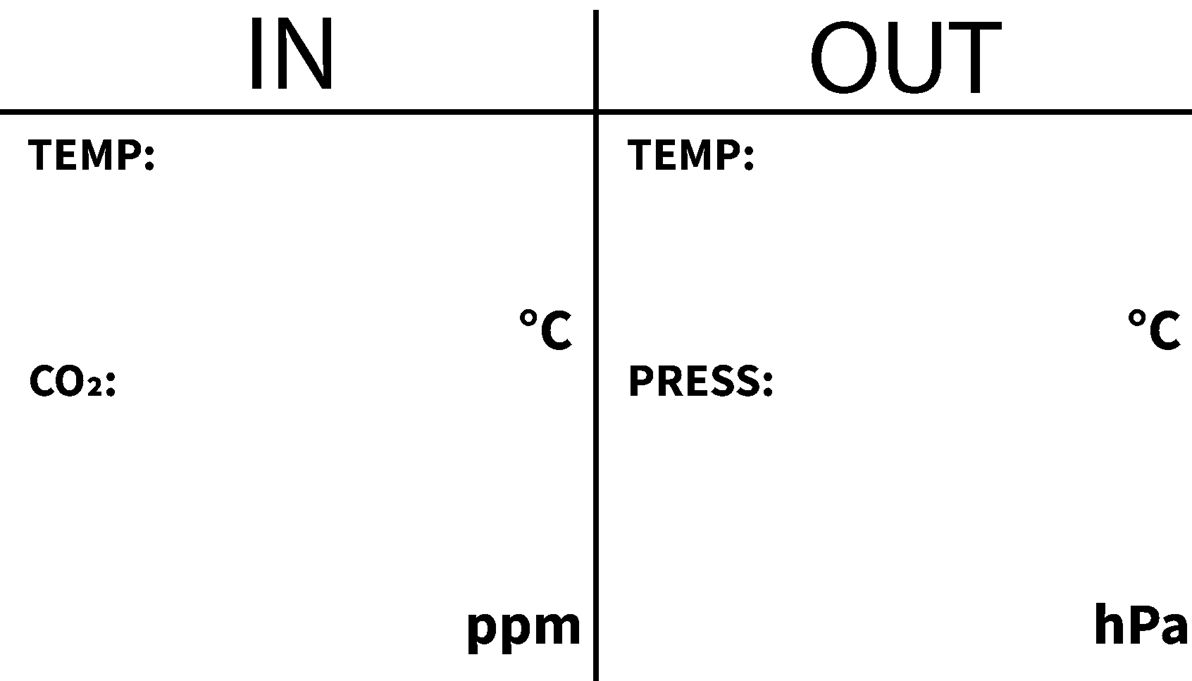
\includegraphics{LaTeX sablona IB/obrazky/PozadiDispleje.png}}
            \caption{Pozadí displeje meteostanice}
            \label{Pozadi}
            \end{figure}
            
            \begin{figure}[htb]
            \resizebox{10cm}{!}{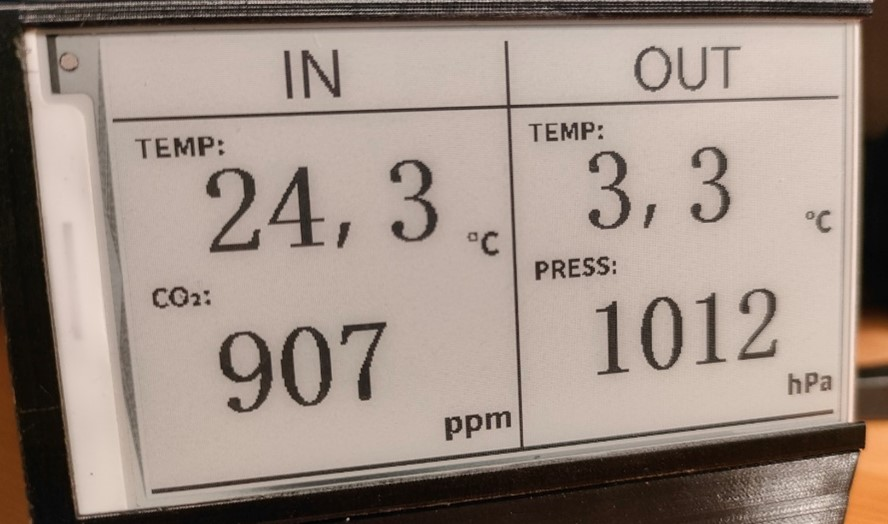
\includegraphics{LaTeX sablona IB/obrazky/DisplejShodnotami.jpg}}
            \caption{Displej s vykreslenými hodnotami}
            \label{Displej}
            \end{figure}

        \clearpage

            Další část programování, se kterou jsem strávil dost času bylo zapisování dat na paměťovou kartu. To probíhá ve funkci \hbox{write\_Data()}, kde se funkcí getTime() nejdříve zjistí a zapíše datum a čas. Funkce getTime() také vytvoří cestu a název souboru, protože soubory se jmenují dle data (například \hbox{23\_02\_2024.txt)} a nachází se ve složkách s názvem podle měsíce a roku. Na každý měsíc tedy připadá jedna složka. Po funkci getTime() se všechny hodnoty zapíší do proměnné ZAPIS datového typu const char* funkcí sprintf() a proměnná ZAPIS se připíše do souboru za datum a čas. Příklad takového zápisu je na obrázku~\ref{Zapis}. Ve funkci \hbox{write\_Data()} se také přepisují maximální a minimální hodnoty venkovní teploty, vlhkosti a tlaku.

            \begin{figure}[htb]
            \resizebox{12.5cm}{!}{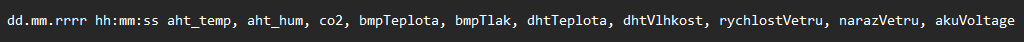
\includegraphics{LaTeX sablona IB/obrazky/info.png}}
            \caption{Soubor info.txt}
            \label{Info}
            \end{figure}

            \begin{figure}[htb]
            \resizebox{12.5cm}{!}{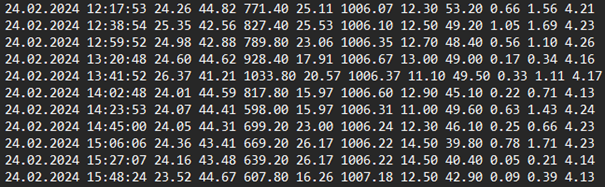
\includegraphics{LaTeX sablona IB/obrazky/ZapisDat.png}}
            \caption{Ukázka zápisu na SD}
            \label{Zapis}
            \end{figure}

            Třetí zásadní část programování je funkčnost a vzhled webserveru. Vše týkající se webserveru je v hlavičkovém souboru Webserver.h. Velkou část tohoto souboru tvoří samotný HTML kód a v další části je funkce Alojz(), která získává jednoduchou předpověď počasí. Webová stránka, viz obrázek~\ref{obr:web}, se dělí na 4 bloky hodnot. Hned pod nadpisem se nachází předpověď a~pod předpovědí jsou aktuální data z meteostanice rozdělena do dvou sloupců (vnitřní a venkovní). Ve sloupečku vnitřních hodnot se nachází také indikátor SD karty, pokud je zelený, vše funguje tak, jak má. Červená znamená chybu zápisu, nebo že karta není vložena. Pod aktuálními hodnotami je tabulka maximálních a minimálních hodnot venkovní teploty, vlhkosti a tlaku a dole vlevo jsou základní informace o chodu meteostanice (uběhlý čas od posledního příjmu hodnot z venkovní jednotky, stav akumulátoru a datum spuštění).

            \begin{figure}[htb]
            \resizebox{12.5cm}{!}{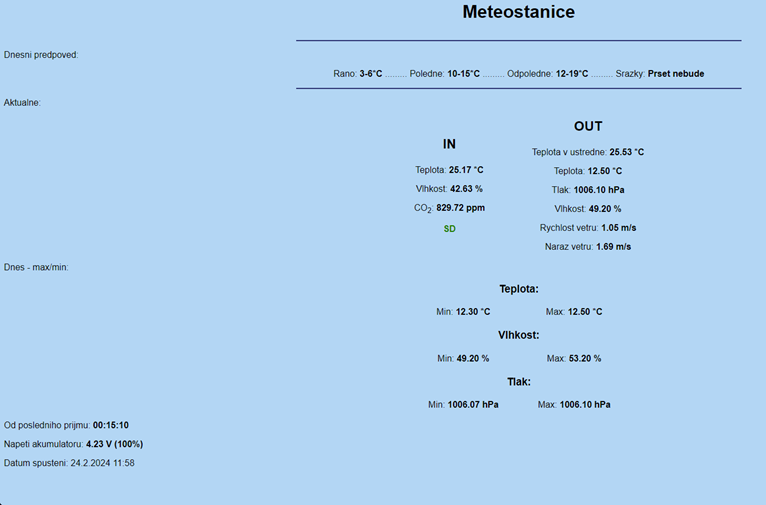
\includegraphics{LaTeX sablona IB/obrazky/Webserver.png}}
            \caption{Vzhled webové stránky}
            \label{obr:web}
            \end{figure}

        \clearpage
        \chapter{Vyhodnocení} \label{Vyhodnoceni}
    Obě jednotky meteostanice jsem testoval v průběhu výroby. vnitřní i venkovní jednotku jsem několikrát nechal společně běžet celý den, někdy i přes víkend. V průběhu jsem kontroloval zápis na paměťovou kartu a vylepšoval vzhled a vlastnosti webserveru. Kalibraci anemometru jsem prováděl pomocí vypůjčeného anemometru, který byl součástí sady Voltcraft UM5/1 100. Měření jsem provedl vícekrát a pokaždé s jinou rychlostí větru. Při každém měření vyšla odchylka trochu jinak. Přibližně se z toho ale dá určit konstanta 2,7 pro korekci rychlosti větru. Během měření se tedy naměřená rychlost otáčení vrtulky vynásobí touto konstantou a vyjde přibližná rychlost větru.

    Venkovní i vnitřní jednotka fungují podle zadání, dosah rádiové komunikace je dostatečný. Akumulátor se při chodu stíhá dobíjet solárním panelem. Vnitřní jednotka zpracovává a zobrazuje data. Anemometr se točí nad má očekávání, ložisko má velmi nízké tření. S radiačním krytem jsem také spokojený, myslím, že plní svůj účel. I přes všechny tyto úspěchy je tu však samozřejmě několik věcí, které by se daly vylepšit nebo přidat. Z~těch hlavních  mi na meteostanici chybí měření úhrnu srážek a měření směru větru. Dále by se také dalo vylepšit zpracování i zobrazení naměřených dat (například nějaké grafy). 

    Do obou jednotek jsem chtěl přidat možnost připojit NTC teplotní čidlo, kdyby bylo potřeba měřit na dalším místě. Hlavně u vnitřní jednotky by to bylo užitečné. Narazil jsem ale na problém s AD převodníkem. U obou mikrokontrolerů ESP32 je velmi nepřesný. Šum pomohl vyřešit kondenzátor a průměrování několika naměřených hodnot. ADC ale není po celém rozsahu dokonale lineární. Při měření napětí akumulátoru to není takový problém. Akumulátor je připojený přes odporový dělič 1:2 a napětí na GPIO pinu tedy nabývá hodnot od 1,85 do 2,1 V, což je ještě v prostředním pásmu, kde je charakteristika ADC lineární. I tak je potřeba k hodnotě přičíst konstantu, protože je zde mírný offset. při měření odporu NTC čidla by se napětí pohybovalo ve větším rozsahu a jednoduchá konstanta pro korekci už by nestačila. Řešením je vytvořit takzvanou Look Up Table, která by každou hodnotu z ADC ($2^{12}$) přiřadila ke správné hodnotě napětí.
        \chapter{Závěr}
    Cílem této práce bylo navrhnout, zkonstruovat a naprogramovat meteostanici, která měří základní meteorologické veličiny. Meteostanice měří vnitřní a~venkovní teplotu, vnitřní a venkovní vlhkost, koncentraci $CO_2$, atmosférický tlak, rychlost větru a stav akumulátoru. Naměřená data zpracovává, zapisuje na paměťovou kartu a zobrazuje na displeji i webserveru. Splňuje tedy zadání. S~výsledkem jsem spokojený, avšak je tu dost věcí, které bych chtěl do budoucna přidat či vylepšit. Po tomto školním roce plánuji mít meteostanici doma na zahradě a dále ji vyvíjet po hardwarové i softwarové stránce. Do budoucna bych chtěl přidat například část na měření úhrnu srážek. Tento senzor funguje na principu kolébky, do které stéká voda z~nálevky. Když se půlka kolébky naplní, překlopí se a plní se druhá půlka. Při každém překlopení by se magnet na kolébce přiblížil ke stejnému senzoru jako v~anemometru. Podle počtu pulzů, času, prostoru nálevky a objemu kolébky by bylo možné vypočítat aktuální úhrn srážek za nějaký čas. Dále bych rád přidal měření směru větru a naprogramoval LUT (Look Up Table) pro zpřesnění měřených hodnot ADC. Práce na tomto projektu mi zcela jistě přinesla mnoho zkušeností, ať už v elektronice, programování, nebo 3D návrhu. Zlepšil jsem se v~modelování i~v~samotném návrhu a konstruování. I když to možná nevypadá, vývojem této meteostanice jsem strávil neskutečné množství času. A tak doufám a věřím, že jsem při tom zlepšil své schopnosti a naučil se něco nového a užitečného.

\pagestyle{plain}
	
\begin{thebibliography}{99}
%1
\bibitem{JakVybratCHytrouMeteostanici} Jiří V. Matýsek. {\it Jak vybrat (chytrou) meteostanici?}. Internetový článek. Dostupné z: \url{https://www.alza.cz/jak-vybrat-chytrou-meteostanici} [cit.~2024-02-28].

%2
\bibitem{ChytraPetr} Bc. Petr Chytra. {\it Návrh a realizace mobilní meteostanice}. Diplomová práce. Dostupné z: \url{https://theses.cz/id/sv3z0w/Chytra_Petr_2022_DP.pdf} [cit.~2024-02-28].

%3
\bibitem{Meteostanice} {\it Meteostanice}. Internetový článek. Dostupné z: \url{https://www.alza.cz/meteostanice/18851185.htm} [cit.~2024-02-28].

%4
\bibitem{HyundayWS2303} {\it Meteorologická stanice Hyundai WS 2303}. Internetová stránka. Dostupné z: \url{https://www.hyundai-electronics.cz/products/meteorologicka-stanice-hyundai-ws-2303-cerna-hyuws2303} [cit.~2024-02-28].

%5
\bibitem{WS2303Obrazek} {\it Hyundai WS 2303}. Obrázek. Dostupné z: \url{https://www.bscom.cz/meteostanice-hyundai-ws-2303-cerna-hyuws2303_d586073/} [cit.~2024-02-28].

%6
\bibitem{SWS12500WIFI} {\it SWS 12500 WIFI
WIFI PROFESIONÁLNÍ METEOROLOGICKÁ STANICE}. Internetová stránka. Dostupné z: \url{https://www.sencor.cz/profesionalni-meteorologicka-stanice/sws-12500?gclid=Cj0KCQjwhL6pBhDjARIsAGx8D5_3TnIyIIkx4KSE45aMHz_K934oUZaL_29lp6ClvO734jhufebWV7waApUaEALw_wcB} [cit.~2024-02-28].

%7
\bibitem{SWS12500Obrazek} {\it SWS 12500 WIFI}. Obrázek. Dostupné z: \url{https://www.sencor.cz/Sencor/media/static-media/8c5ee219-66e4-4da8-8fc1-e87f2de5c32d@w800.webp} [cit.~2024-02-28].

%8
\bibitem{DisplejToply} Jan Šimečík. {\it Displej: Jak vlastně funguje a jaké jsou jeho typy a parametry?}. Internetový článek. Dostupné z: \url{https://toply.cz/pojmy/displej/} [cit.~2024-02-28].

%9
\bibitem{ElektromechanickeDispleje} {\it Elektromechanické displeje}. Internetový článek. Dostupné z: \url{http://www.plc-automatizace.cz/knihovna/hmi/technologie/mechanicke.htm} [cit.~2024-02-28].

%10
\bibitem{ZobrazovaciJednotky} {\it Zobrazovací jednotky}. Internetový článek. Dostupné z: \url{http://old.spsemoh.cz/vyuka/zel/zobrazovaci-jednotky.htm} [cit.~2024-02-28].

%11
\bibitem{LCDsegDisplej} {\it Kladný 7 segmentový TN LCD displej}. Obrázek. Dostupné z: \url{https://sk.enrichlcddisplay.com/lcd/segment-lcd/positive-7-segment-tn-lcd-panel-display.html} [cit.~2024-02-28].

%12
\bibitem{7segmentdisplejPrincipAfunkcia} 
Elektrolab. {\it ROZDELENIE, PRINCÍP A FUNKCIA 7 SEGMENTOVÉHO DISPLEJA}. Internetový článek. Dostupné z: \url{https://www.elektrolab.eu/blog/rozdelenie-princip-a-funkcia-7-segmentoveho-displeja} [cit.~2024-02-28].

%13
\bibitem{MaticovyLEDdisplej} Martin Sejkora. {\it Maticový LED displej}. Středoškolská technika 2016, ČVUT. Dostupné z: \url{http://stretech.fs.cvut.cz/2016/sbornik_2016/a-CD-stretech2016/Pardubice-Sejkora-Maticový%20displej.pdf} [cit.~2024-02-28].

%14
\bibitem{MaticovyDisplej} {\it Maticový displej}. Obrázek. Dostupné z: \url{https://www.tetronik.cz/produkty/produkt/6_displeje?parent=1} [cit.~2024-02-28].

%15
\bibitem{DisplejeLCD} {\it Displeje LCD}. Internetový článek. Dostupné z: \url{https://eluc.ikap.cz/verejne/lekce/627} [cit.~2024-02-28].

%16
\bibitem{ZobrazovaciGrafickaZarizeni} Michal Křížek. {\it Zobrazovací grafická zařízení}. Bakalářská práce. Dostupné z: \url{https://theses.cz/id/fegqtw/69380-157735417.pdf} [cit.~2024-02-28].

%17
\bibitem{TFTLCDdisplej} {\it 5" palcový TFT LCD displej 800x480 40pin dotyk}. Obrázek. Dostupné z: \url{https://www.briv.cz/p/5128/5-palcovy-tft-lcd-displej-800x480-40pin-dotyk} [cit.~2024-02-28].

%18
\bibitem{OLEDDisplay} {\it EA OLEDL128-6GGA - OLED Display 128 x 64 Žlutý, Display Visions}. Obrázek. Dostupné z: \url{https://www.distrelec.cz/cs/oled-display-128-64-zluty-display-visions-ea-oledl128-6gga/p/30108668} [cit.~2024-02-28].

%19
\bibitem{EinkToply} Jan Šimečík. {\it Elektronický papír: Co je e-ink displej a jaké je jeho využití?}. Internetový článek. Dostupné z: \url{https://toply.cz/ctecky-knih/elektronicky-papir-e-ink/} [cit.~2024-02-28].

%20
\bibitem{E-Ink800x480px} {\it E-Ink 7,5"800x480px}. Obrázek. Dostupné z: {\tt https://botland.cz/e-papir-displeje/9891-e-papir-e-ink-75\\-800x480px-displej-s-prekrytim-hat-pro-raspberry-pi-\\waveshare-13504-5904422338558.html} [cit.~2024-02-28].

%21
\bibitem{ONYXBOOXMIRAPRO} {\it ONYX BOOX MIRA PRO 25,3"}. Obrázek. Dostupné z: \url{https://www.ebook-ctecky.cz/onyx-boox-mira-pro-25-3-stojan#tb1=1} [cit.~2024-02-28].

%22
\bibitem{Mereniteploty} {\it Měření teploty}. Internetový článek. Dostupné z: \url{https://uprt.vscht.cz/kminekm/mrt/F4/F4k43-tepl.htm} [cit.~2024-02-28].

%23
\bibitem{AutodeskFusion360} Autodesk. {\it Autodesk Fusion 360}. Software. Dostupné z: \url{https://www.autodesk.cz/products/fusion-360/overview?term=1-YEAR&tab=subscription} [cit.~2024-02-28].

%24
\bibitem{KiCad} {\it KiCad 7.0}. Software. Dostupné z: \url{https://www.kicad.org} [cit.~2024-02-28].

%25
\bibitem{A3144Hall} {\it A3144 Hall Effect Sensor Pinout}. Obrázek. Dostupné z: \url{https://www.jakelectronics.com/subject/a3144-hall-effect-sensor-datasheet-circuit-and-pinout} [cit.~2024-02-28].

%26
\bibitem{ArduinoIDE} Arduino. {\it Arduino IDE 2.3.2}. Software. Dostupné z: \url{https://www.arduino.cc/en/software} [cit.~2024-02-28].

%27
\bibitem{Illustrator} Adobe. {\it Adobe Illustrator}. Software. Dostupné z: \url{https://www.adobe.com/cz/products/illustrator.html} [cit.~2024-02-28].

%28
\bibitem{Image2Lcd} {\it Image2Lcd Ver3.2}. Software. Dostupné z: \url{https://www.e-paper-display.com/download_detail/downloadsId=625.html} [cit.~2024-02-28].

%29
\bibitem{Wire} {\it Wire}. Knihovna. Dostupné z: \url{https://www.arduino.cc/reference/en/language/functions/communication/wire/} [cit.~2024-02-28].

%30
\bibitem{AdafruitSensor} Adafruit Industries. {\it \hbox{Adafruit\_Sensor}}. Knihovna. Dostupné z: \url{https://github.com/adafruit/Adafruit_Sensor/blob/master/Adafruit_Sensor.h} [cit.~2024-02-28].

%31
\bibitem{AdafruitBMP280Library} Adafruit Industries. {\it \hbox{Adafruit\_BMP280\_Library}}. Knihovna. Dostupné z: \url{https://github.com/adafruit/Adafruit_BMP280_Library} [cit.~2024-02-28].

%32
\bibitem{DHTsensorLibrary} {\it DHT sensor library}. Knihovna. Dostupné z: \url{https://www.arduino.cc/reference/en/libraries/dht-sensor-library/} [cit.~2024-02-28].

%33
\bibitem{RHASK} Paul Stoffregen. {\it \hbox{RH\_ASK}}. Knihovna. Dostupné z: \url{https://github.com/PaulStoffregen/RadioHead/blob/master/RH_ASK.h} [cit.~2024-02-28].

%34
\bibitem{SPI} {\it SPI}. Knihovna. Dostupné z: \url{https://www.arduino.cc/reference/en/language/functions/communication/spi/} [cit.~2024-02-28].

%35
\bibitem{WiFi} {\it WiFi}. Knihovna. Dostupné z: \url{https://www.arduino.cc/reference/en/libraries/wifi/} [cit.~2024-02-28].

%36
\bibitem{WiFiClient} Espressif Systems. {\it WiFiClient}. Knihovna. Dostupné z: \url{https://github.com/espressif/arduino-esp32/blob/master/libraries/WiFi/src/WiFiClient.h} [cit.~2024-02-28].

%37
\bibitem{WebServer} Espressif Systems. {\it WebServer}. Knihovna. Dostupné z: \url{https://github.com/espressif/arduino-esp32/blob/master/libraries/WebServer/src/WebServer.h} [cit.~2024-02-28].

%38
\bibitem{ESPmDNS} Espressif Systems. {\it ESPmDNS}. Knihovna. Dostupné z: \url{https://github.com/espressif/arduino-esp32/blob/master/libraries/ESPmDNS/src/ESPmDNS.h} [cit.~2024-02-28].

%39
\bibitem{HTTPClient} Espressif Systems. {\it HTTPClient}. Knihovna. Dostupné z: \url{https://github.com/espressif/arduino-esp32/blob/master/libraries/HTTPClient/src/HTTPClient.h} [cit.~2024-02-28].

%40
\bibitem{FS} Espressif Systems. {\it FS}. Knihovna. Dostupné z: \url{https://github.com/espressif/arduino-esp32/blob/master/libraries/FS/src/FS.h} [cit.~2024-02-28].

%41
\bibitem{SD} Arduino Libraries. {\it SD}. Knihovna. Dostupné z: \url{https://github.com/arduino-libraries/SD} [cit.~2024-02-28].

%42
\bibitem{time} {\it time}. Knihovna. Dostupné z: \url{https://www.tutorialspoint.com/c_standard_library/time_h.htm} [cit.~2024-02-28].

%43
\bibitem{ErriezMHZ19B} Erriez. {\it ErriezMHZ19B}. Knihovna. Dostupné z: \url{https://github.com/Erriez/ErriezMHZ19B} [cit.~2024-02-28].

%44
\bibitem{AHTxx} enjoyneering. {\it AHTxx}. Knihovna. Dostupné z: \url{https://github.com/enjoyneering/AHTxx/blob/main/src/AHTxx.h} [cit.~2024-02-28].

%45
\bibitem{Alojz} {\it Alojz}. Internetová stránka. Dostupné z: \url{https://alojz.cz/praha} [cit.~2024-02-28].

%46
\bibitem{EpaperLibrary} GoodDisplay. {\it E-Paper Library}. Ukázkový kód. Dostupné z: \url{https://www.good-display.com/companyfile/24/} [cit.~2024-02-28].

\end{thebibliography}
\appendix
    \chapter{Obsah přiloženého .zip souboru}

        /trnkaja20 \newline
        .\hspace{1cm}/elektro\newline
        .\hspace{2cm}\hbox{dokumentace\_DPS.pdf}\newline
        .\hspace{2cm}\hbox{pcb\_DHT22.zip}\newline
        .\hspace{2cm}\hbox{pcb\_venkovni.zip}\newline
        .\hspace{2cm}\hbox{pcb\_vnitrni.zip}\newline
        .\hspace{2cm}\hbox{schema\_zapojeni\_venkovni\_jednotka.png}\newline
        .\hspace{2cm}\hbox{schema\_zapojeni\_vnitrni\_jednotka.png}\newline
        .\hspace{1cm}/media\newline
        .\hspace{2cm}\hbox{foto\_venkovni\_jednotka.jpg}\newline
        .\hspace{2cm}\hbox{foto\_vnitrni\_jednotka.jpg}\newline
        .\hspace{2cm}\hbox{foto\_zapojeni\_venkovni.jpg}\newline
        .\hspace{2cm}\hbox{foto\_zapojeni\_vnitrni.jpg}\newline
        .\hspace{2cm}\hbox{screenshot\_webserver.png}\newline
        .\hspace{2cm}\hbox{video\_funkcnosti.mp4}\newline
        .\hspace{1cm}/mechanika\newline
        .\hspace{2cm}\hbox{3d\_modely.zip}\newline
        .\hspace{1cm}/program\newline
        .\hspace{2cm}/knihovny\newline
        .\hspace{2cm}\hbox{program\_venkovni\_ESP32c3.zip}\newline
        .\hspace{2cm}\hbox{program\_vnitrni\_ESP32s3.zip}\newline
        .\hspace{1cm}trnkaja20.pdf\newline
        .\hspace{1cm}trnkaja20.zip\newline
        .\hspace{1cm}\hbox{trnkaja20\_ekonomicka\_cast.xlsx}\newline
        
        \clearpage
        
    \chapter{Blokové schéma zapojení}
    
        \begin{figure}[htb]
        \resizebox{12cm}{!}{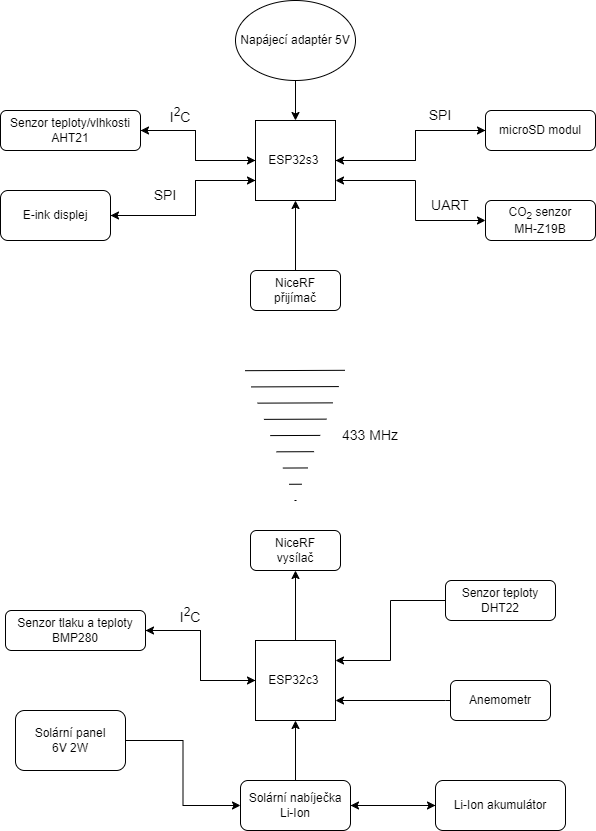
\includegraphics{LaTeX sablona IB/obrazky/SchemaElZapojeni.png}}
        %\caption{popisek}
        %\label{}
        \end{figure}

        \clearpage
        
    \chapter{Vývojový diagram}
        \section{Venkovní jednotka}
            \begin{figure}[htb]
            \resizebox{6cm}{!}{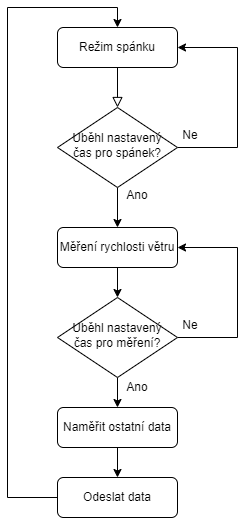
\includegraphics{LaTeX sablona IB/obrazky/vyvojovy_diagram_venkovni.png}}
            %\caption{popisek}
            %\label{}
            \end{figure}

            \clearpage

        \section{Vnitřní jednotka}
            \begin{figure}[htb]
            \resizebox{12.5cm}{!}{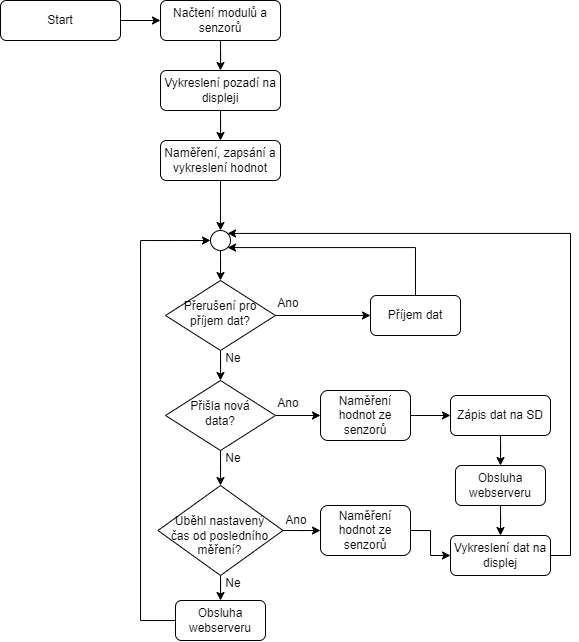
\includegraphics{LaTeX sablona IB/obrazky/vyvojovy_diagram_vnitrni.png}}
            %\caption{popisek}
            %\label{}
            \end{figure}


\end{document}